\documentclass{scrartcl}
%\documentclass{article}
\usepackage[ngerman]{babel}
\usepackage[utf8]{inputenc}
\usepackage{courier}
\usepackage{amsmath}
\usepackage{graphicx}
\usepackage{tabularx}
\usepackage{amssymb}
\usepackage{hyperref}
\usepackage{verbatim}
\usepackage{algorithm}
\usepackage{algorithmic}
\renewcommand{\algorithmiccomment}[1]{\textit{#1}}
\renewcommand{\algorithmicrequire}{\textbf{Eingabe:}} 
\renewcommand{\algorithmicensure}{\textbf{Ausgabe:}}
%\renewcommand{\contentsname}{Inhaltsverzeichnis}
\newcommand{\name}[1]{\textbf{\texttt{#1}}}
\newcommand{\field}[1]{\item \name{#1}}
\newcommand{\property}[1]{\item \name{#1}}
\newcommand{\method}[1]{\item \name{#1}}
%\renewcommand*\rmdefault{ppl}\normalfont\upshape

\begin{document}
\title{
    \hspace{-0.5cm} 
\includegraphics[height=5cm]{logo.png} \\[1cm]
    \Huge{YUV.KA} \\ \large{Praxis der Softwareentwicklung 2011/2012}
}
\author{Max Wagner $\cdot$ Patrick Gemander $\cdot$ Sebastian Ullrich $\cdot$ Michael Vollmer \\ Robert Hangu $\cdot$ Daniel Lebert}
\maketitle

\newpage
\mbox{}
\newpage
\mbox{}

\addcontentsline{toc}{section}{Inhaltsverzeichnis}
\tableofcontents

\section{Namespace-Dependencies}
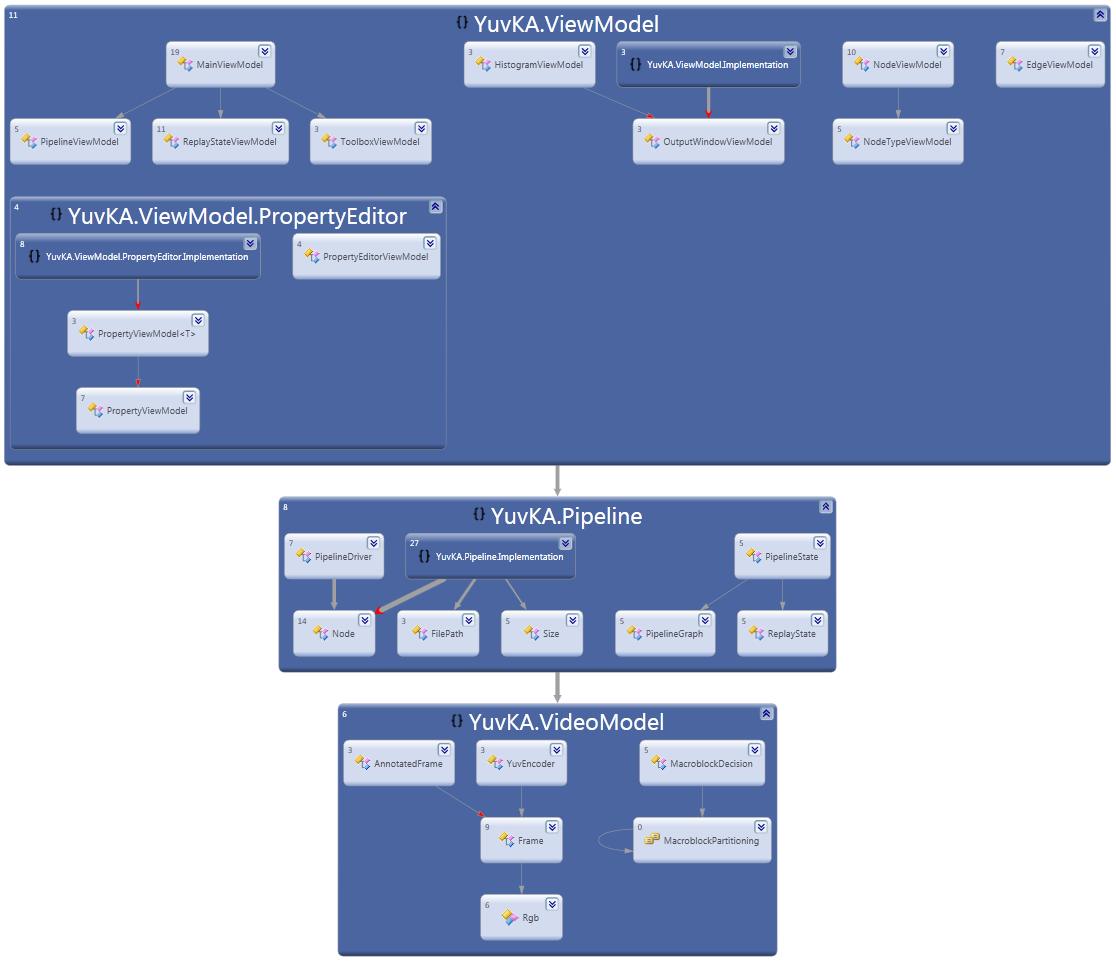
\includegraphics[width=\textwidth]{Diagrams/namespacedependencies.png}
Veranschaulichung der ``Model View ViewModel''-Architektur, die bei diesem Projekt umgesetzt wird. Die ``View'' wird hierbei jedoch nicht dargestellt, da sie selbst keinerlei Logik enthält.
\begin{description}
	\item[VideoModel]~\\
	Das VideoModel repräsentiert ein eingelesenes Video, ggf. mit zugehörigen Log-Daten. Da es die Daten im RGB-Format speichert, müssen diese bei Eingabe und Ausgabe vom bzw. ins YUV-Format konvertiert
werden.

	\item[Pipeline]~\\
	Die Pipeline-Schicht repräsentiert den UI-unabhängigen Aufbau des Analyse-DAGs\footnote{\emph{directed acyclic graph}}. Sie besteht einerseits aus den unterschiedlichen Knoten-Klassen, die unabhängig voneinander ihren jeweiligen Algorithmus auf Frame-für-Frame-Basis implementieren, und andererseits aus dem Pipeline Driver, der für die Abhängigkeitsauflösung und letztendliche Abarbeitung der Pipeline zuständig ist.
	
	\item[ViewModel]~\\
	Nach dem Model-View-ViewModel-Pattern (MVVM) ist es Aufgabe der ViewModel-Schicht, das Model der View in einer für sie verarbeitbaren Form zu präsentieren. Bezogen auf das Projekt bedeutet dies vor allem, die Model-Klassen um View-spezifische Daten (wie Positionierung auf der Oberfläche) und Methoden zu ergänzen.

\end{description}




\clearpage

\section{YuvKA.VideoModel}
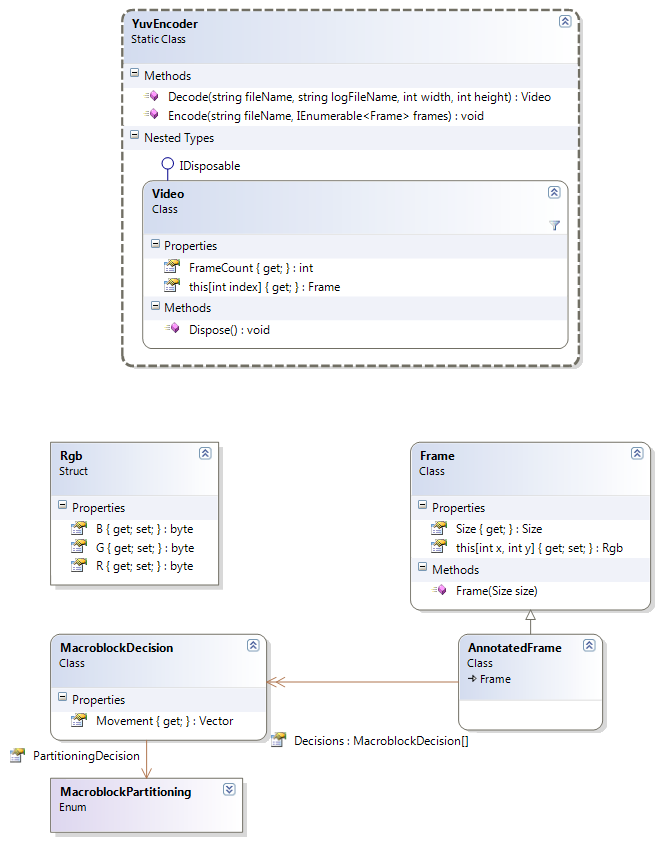
\includegraphics[width=\textwidth]{YuvKA.VideoModel/videomodel.png}
Das \name{VideoModel} besteht aus denjenigen Klassen, die die unterschiedlichen Framearten bilden, einschließlich ihrer Hilfsklassen. Außerdem gehört die Klasse \name{YuvEncoder} mit der inneren Klasse \name{Video} dazu, die Videos vom YUV-Format ins RGB-Format umwandelt, mit der das Programm intern arbeitet.

\subsubsection{YuvKA.VideoModel.YuvEncoder}

\begin{verbatim}
public static class YuvEncoder
\end{verbatim}

\paragraph{Beschreibung}~\\
Die Klasse \name{YuvEncoder} bietet die Funktionalität, Videos, die im YUV-Format eingegeben werden, ins RGB-Format umzuwandeln, damit das Programm damit arbeiten kann. Des Weiteren wandelt sie die manipulierten Videos vom RGB-Format ins YUV-Format um, damit sie abgespeichert werden können.

\paragraph{Typmember}
\begin{itemize}

\method{Decode}
	\begin{verbatim}
	public static Video Decode(string fileName, string logFileName,
    int width, int height)
	\end{verbatim}
	Wandelt das im \name{fileName} angegebene YUV-Video ins RGB-Format um, das interne Format des Programms. Falls der Parameter \name{logFileName} nicht \name{null} ist, werden die \name{Frame}s mit entsprechendem Log als \name{AnnotatedFrame}s ausgegeben.

\method{Encode}
	\begin{verbatim}
	public static void Encode(string fileName,
    IEnumerable<Frame> frames)
	\end{verbatim}
	Wandelt das als RGB-Frameliste angegeben Video ins YUV-Format um und speichert es unter \name{fileName}. 

\end{itemize}

\setcounter{secnumdepth}{4}
\paragraph{YuvKA.VideoModel.YuvEncoder.Video}
\setcounter{secnumdepth}{3}

\begin{verbatim}
public class Video : IDisposable
\end{verbatim}

\paragraph{Beschreibung}~\\
Die Klasse \name{Video} hält die vom \name{YuvEncoder} umgewandelten Videos als Videostream.

\paragraph{Typmember}
\begin{itemize}

\property{FrameCount}
	\begin{verbatim}
	public int FrameCount { get; }
	\end{verbatim}
	Ruft die Anzahl der \name{Frame}s im \name{stream} ab.

\property{this[int index]}
	\begin{verbatim}
	public Frame this[int index] { get; }
	\end{verbatim}
	Ruft den an der Stelle \name{index} abgespeicherten \name{Frame} im \name{stream} ab.

\method{Dispose}
	\begin{verbatim}
	public void Dispose()
	\end{verbatim}
	Schließt den \name{stream} des \name{Video}-Objekts, sodass das File-Handle freigegeben wird.

\end{itemize}

\subsubsection{YuvKA.VideoModel.Frame}

\begin{verbatim}
public class Frame
\end{verbatim}

\paragraph{Beschreibung}~\\
Die Klasse \name{Frame} stellt ein Einzelbild eines Videostreams im RGB-Format dar.

\paragraph{Typmember}
\begin{itemize}

\property{Size}
	\begin{verbatim}
	public Size Size { get; }
	\end{verbatim}
	Ruft die Auflösung des \name{Frame}s ab.

\property{this[int x, int y]}
	\begin{verbatim}
	public Rgb this[int x, int y] { get; set; }
	\end{verbatim}
	Ruft den Farbwert des \name{Frame}s an der Stelle \name{x,y} in RGB ab oder legt ihn fest.

\end{itemize}

\subsubsection{YuvKA.VideoModel.AnnotatedFrame}

\begin{verbatim}
public class AnnotatedFrame : Frame
\end{verbatim}

\paragraph{Beschreibung}~\\
Die Klasse \name{AnnotedFrame} erweitert die Klasse \name{Frame} um die Funktion, Logfiles des Encoders zu halten.

\paragraph{Typmember}
\begin{itemize}

\property{Decisions}
	\begin{verbatim}
	public MacroblockDecision[] Decisions { get; }
	\end{verbatim}
	Ruft die Entscheidungen, die der Encoder bei der Kodierung getroffen hat, als Array von \name{MacroblockDecision}-Objekten ab.

\end{itemize}

\subsubsection{YuvKA.VideoModel.MacroblockDecision}

\begin{verbatim}
public class MacroblockDecision
\end{verbatim}

\paragraph{Beschreibung}~\\
Die Klasse \name{MacroblockDecision} stellt die Entscheidung dar, die der Encoder bei der Enkodierung eines Makroblocks getroffen hat.

\paragraph{Typmember}
\begin{itemize}

\property{Movement}
	\begin{verbatim}
	public Vector Movement { get; }
	\end{verbatim}
	Ruft den Bewegungsvektor des Makroblocks relativ zum vorherigen Frame ab.

\property{PartitioningDecision}
	\begin{verbatim}
	public MacroblockPartitioning PartitioningDecision { get; }
	\end{verbatim}
	Ruft die Entscheidung darüber, welche \name{MacroblockPartitioning} bei der Kodierung verwendet wurde ab.

\end{itemize}

\subsubsection{YuvKA.VideoModel.MacroblockPartitioning}

\begin{verbatim}
public enum MacroblockPartitioning
{
    InterSkip, Inter16x16, Inter16x8, Inter8x16,
    Inter8x8, Inter8x4, Inter4x8, Inter4x4,
    Inter8x8OrBelow, Intra4x4, Intra16x16, Intra8x8,
    IntraPCM, Unknown
}
\end{verbatim}
Die \name{MacroblockPartitioning} gibt die verschiedenen Möglichkeiten der Partitionierung eines Makroblocks als Inter- bzw. Intraframe an.

\clearpage

\section{YuvKA.Pipeline}
\subsection{YuvKA.Pipeline.PipelineDriver}

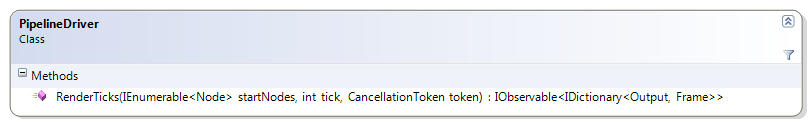
\includegraphics[width=\textwidth]{YuvKA.Pipeline/driver.png}
\begin{verbatim}
public static class PipelineDriver
\end{verbatim}

\paragraph{Beschreibung}~\\
Die Klasse \name{PipelineDriver} ist für die Ausführung der Pipeline zuständig. Sie löst die gegenseitigen Abhängigkeiten der \name{Node}-Instanzen auf, um dann in Reihenfolge einer topologischer Sortierung deren \name{ProcessFrame}-Methoden aufrufen zu können.
Die Klasse soll möglichst parallel implementiert werden, sodass mehrere aufeinanderfolgende Ticks gleichzeitig berechnet werden.

\paragraph{Typmember}
\begin{itemize}

\property{RenderFrames}
	\begin{verbatim}
public static IObservable<IDictionary<Node.Output, Frame>> RenderFrames(
    IEnumerable<Node> startNodes, int tick, CancellationToken token)
    \end{verbatim}
	Berechnet die Pipeline ab dem angegebenen Tick und liefert eine asynchrone Aufzählung zurück, die pro Tick ein Dictionary enthält, das jedem Ausgang der gegebenen Knoten \name{startNodes} den jeweils berechneten Frame zuordnet.

    Parallelitätszusicherungen: Die Methode führt auf einer \name{Node}-Instanz \name{ProcessFrame} immer seriell mit strikt aufsteigendem Tick aus. Die gleiche Ordnung gilt für den Rückgabewert. Die Berechnung wird bei Aktivierung des \name{token}s am nächstmöglichen Punkt beendet.

\end{itemize}

\subsection{Zustandshaltung der Pipeline}

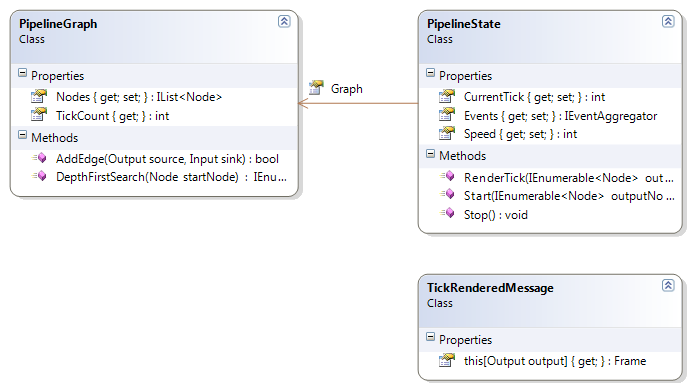
\includegraphics[width=\textwidth]{YuvKA.Pipeline/states.png}
Diese Gruppe von Klassen dient dazu, den Zustand der Pipeline zu verwalten. Der \name{PipelineState} benutzt zur Verwaltung der im Pipeline-Graphen vorhandenen Knoten und Kanten den \name{PipelineGraph}. Er ist zudem dafür zuständig, die Berechnung der Pipeline zu starten und zu stoppen. Die \name{TickRenderedMessage} wird geworfen, wenn ein Zeitabschnitt berechnet ist.

\subsubsection{YuvKA.Pipeline.PipelineState}

\begin{verbatim}
[DataContract]
public class PipelineState
\end{verbatim}

\paragraph{Beschreibung}~\\
Die Klasse \name{PipelineState} vereint in sich den Gesamtzustand des Datenmodells, womit durch ihre Serialisierung alle relevanten Programmdaten gespeichert werden. Sie enthält den aktuellen Wiedergabestatus und bietet zur Wiedergabe eine Schnittstelle zum \name{PipelineDriver}.

\paragraph{Typmember}
\begin{itemize}

\property{CurrentTick}
	\begin{verbatim}
	[DataMember]
	public int CurrentTick { get; set; }
	\end{verbatim} 
	Ruft den nächstes zu berechnenden Tick ab oder legt ihn fest. Das Neusetzen der Property führt zum Abbruch der Berechnung des aktuellen Ticks.

\property{Speed}
	\begin{verbatim}
	[DataMember]
	public int Speed { get; set; }
	\end{verbatim}
	Ruft die Abspielgeschwindigkeit in Frames pro Sekunde ab oder legt sie fest.

\property{Graph}
	\begin{verbatim}
	[DataMember]
	public PipelineGraph Graph { get; }
	\end{verbatim}
	Ruft den \name{PipelineGraph} ab, der die Struktur der Pipeline repräsentiert.

\property{Events}
	\begin{verbatim}
	[Import(typeof(IEventAggregator))]
	public IEventAggregator Events { get; set; }
	\end{verbatim}
	Per Dependency Injection injizierte Schnittstelle zum Caliburn Message System, über das die Ausgabefenster über die Beendigung aller im aktuellen Tick berechneten \name{Frame}s benachrichtigt werden.

\method{Start}
	\begin{verbatim}
	public void Start(IEnumerable<Node> outputNodes)
	\end{verbatim}
	Weist den \name{PipelineDriver} an, die Pipeline ab dem aktuellen Tick für die gegebenen Knoten zu berechnen. Pro abgeschlossener Berechnung eines Ticks wird eine \name{TickRenderedMessage} geworfen.

\method{Stop}
	\begin{verbatim}
	public void Stop()
	\end{verbatim}
	Beendet die Wiedergabe und stoppt den \name{PipelineDriver}. Danach vom \name{PipelineDriver} asynchron erhaltene \name{Frame}s werden ignoriert.

\method{Stop}
	\begin{verbatim}
	public void RenderTick(IEnumerable<Node> outputNodes)
	\end{verbatim}
	Weist den \name{PipelineDriver} an, die Pipeline für den aktuellen Tick und die gegebenen Knoten zu berechnen. Bei abgeschlossener Berechnung wird eine \name{TickRenderedMessage} geworfen.
\end{itemize}

\subsubsection{YuvKA.Pipeline.PipelineGraph}
	
\begin{verbatim}
[DataContract]
public class PipelineGraph	
\end{verbatim}

\paragraph{Beschreibung}~\\
Die Klasse \name{PipelineGraph} verwaltet den Aufbau des Pipeline-Graphen. 
	
\paragraph{Typmember}
\begin{itemize}

\property{Nodes}
	\begin{verbatim}
	[DataMember]
	public IList<Node> Nodes { get; }
	\end{verbatim}
	Verwaltet die im Pipeline-Graphen verfügbaren Knoten und ruft sie ab.

\property{FrameCount}
	\begin{verbatim}
	[DataMember]
	public int FrameCount { get; }
	\end{verbatim}
	Ruft die maximale Länge aller als Input gegebenen Videos ab.


	
\method{AddEdge}
	\begin{verbatim}
	public bool AddEdge(Output source, Input sink)
	\end{verbatim}
	Wenn die durch \name{source} und \name{sink} spezifizierte Kante zu keinem Zyklus innerhalb des Pipeline-Graphen führt, so soll sie durch setzen der Output-Property von \name{source} als \name{sink} hinzugefügt und true ausgegeben werden. Andernfalls soll die Kante nicht zum Graphen hinzugefügt und false ausgegeben werden.
\end{itemize}
	
\subsubsection{YuvKA.Pipeline.TickRenderedMessage}
		
\begin{verbatim}
public class TickRenderedMessage
\end{verbatim}

\paragraph{Beschreibung}~\\
Die Klasse \name{TickRenderedMessage} enthält die im letzten Tick berechneten \name{Frame}s aller \name{Output}s.

\paragraph{Typmember}
\begin{itemize}
	
\property{this[]}
	\begin{verbatim}
	public Frame this[Output output] { get; }
	\end{verbatim}
Indexer. Ruft den durch \name{output} spezifizierten \name{Frame} auf.

\end{itemize}

\subsection{Node}
\begin{center}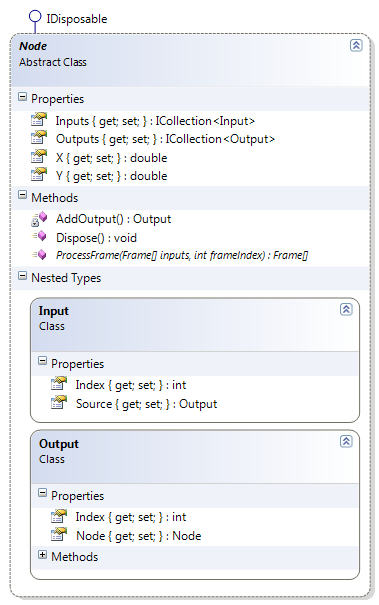
\includegraphics[scale=0.7]{YuvKA.Pipeline/node.png} \\
\end{center}
Die Basisklasse \name{Node} stellt die Attribute und Methoden zur Verfügung, welche von allen Knoten (seien dies Eingabe-, Ausgabe- oder Manipulationsknoten) benötigt werden. Dies umfasst die \name{Process}-Methode, welche die tatsächliche Bearbeitung der \name{Frame}s darstellt, als auch alle Informationen bezüglich der Verbindungen zwischen verschiedenen Knoten, welche in den inneren Klassen \name{Input} und \name{Output} gestellt sind.

\subsubsection{YuvKA.Pipeline.Node}

\begin{verbatim}
[InheritedExport]
[DataContract]
public abstract class Node : IDisposable
\end{verbatim}

\paragraph{Beschreibung}~\\
Die abstrakte Klasse \name{Node} stellt die gemeinsame Struktur aller Knoten zur Verfügung. Die allgemeine Arbeitsweise eines solchen Knotens besteht darin, dass er nach seiner Konstruktion und dem Verbinden seiner Eingänge (falls er welche hat) durch einen Aufruf der Funktion \name{Process} zur Verarbeitung der gegebenen \name{Frame}s ab dem gegebenen Index gebracht wird. Was die Bearbeitung beinhaltet wird in der jeweiligen Unterklasse spezifiziert.

\paragraph{Typmember}
\begin{itemize}

\property{X}
	\begin{verbatim}
	[Browsable(false)]
	[DataMember]
	public double X { get; set; }
	\end{verbatim}
	Stellt die X-Koordinate des Knoten im Graphen dar.

\property{Y}
	\begin{verbatim}
	[Browsable(false)]
	[DataMember]
	public double Y { get; set; }
	\end{verbatim}
	Stellt die Y-Koordinate des Knoten im Graphen dar.

\property{Inputs}
	\begin{verbatim}
[Browsable(false)]
public ICollection<Input> Inputs { get; private set; }
	\end{verbatim}
Stellt die Eingänge eines Knoten dar. Siehe innere Klasse \name{Input}

\property{Outputs}
	\begin{verbatim}
[Browsable(false)]
public ICollection<Output> Outputs { get; private set; }
	\end{verbatim}
Stellt die Ausgänge eines Knoten dar. Siehe innere Klasse \name{Output}

\method{Process}
	\begin{verbatim}
public abstract Frame[] Process(Frame[] inputs, int tick);
	\end{verbatim}
	Verarbeitet die gegebenen \name{Frame}s entsprechend dem internen Algorithmus und gibt ein Array von \name{Frame}s als Resultat zurück. Der Parameter \name{inputs} ist hierbei direkt als die Daten, welche an den Eingängen des Knotens anliegen, zu interpretieren. Dementsprechend entspricht der Rückgabewert den Daten, welche an den Ausgängen des Knotens durchgereicht werden. Verschiedene Knoten überschreiben diese Methode mit verschiedenen Implementationen.


\end{itemize}

\subsubsection{YuvKA.Pipeline.Node.Input}

\begin{verbatim}
public class Input
\end{verbatim}

\paragraph{Beschreibung}~\\
Die innere Klasse \name{Input} stellt einen Eingang eines Knotens dar, von dem der Knoten seine zu verarbeitenden Daten bezieht. (Dies gilt natürlich nicht für Unterklassen der Klasse \name{InputNode}, welche in der Regel keine Eingänge haben und ihre Daten von anderen Stellen beziehen.)

\paragraph{Typmember}
\begin{itemize}

\property{Source}
	\begin{verbatim}
public Output Source { get; set; }
	\end{verbatim}
Enthält die Quelle des Einganges. Graphisch gesehen entspricht dies dem ``Anfang der Kante'' zwischen zwei Knoten.

\property{Index}
	\begin{verbatim}
public int Index { get; }
	\end{verbatim}
Speichert den Index des Einganges. Dies ist insbesondere bei Knoten wichtig, welche einen Unterschied zwischen verschiedenen Eingängen machen (zum Beispiel der \name{DifferenceNode}-Knoten, welcher die Pixeldaten verschiedener Eingänge voneinander subtrahiert).

\end{itemize}


\subsubsection{YuvKA.Pipeline.Node.Output}

\begin{verbatim}
public class Input
\end{verbatim}

\paragraph{Beschreibung}~\\
Die innere Klasse \name{Output} stellt einen Ausgang eines Knotens dar, durch den die verarbeiteten Daten eines Rechenschrittes weitergegeben werden. (Dies gilt natürlich nicht für Unterklassen der Klasse \name{OutputNode}, welche in der Regel keine Ausgänge haben.)

\paragraph{Typmember}
\begin{itemize}

\property{Node}
	\begin{verbatim}
public Node Node { get; }
	\end{verbatim}
Speichert den Knoten, zu dem der Ausgang gehört.

\property{Index}
	\begin{verbatim}
public int Index { get; }
	\end{verbatim}
Speichert den Index des Ausgangs. Dies ist insbesondere bei Knoten wichtig, welche einen Unterschied zwischen verschiedenen Ausgängen machen (zum Beispiel der \name{RgbSplitNode}-Knoten, welcher die Pixeldaten seiner Eingabe in Rot-, Grün- und Blaukanal aufteilt).

\end{itemize}

\subsection{Eingabeknoten}

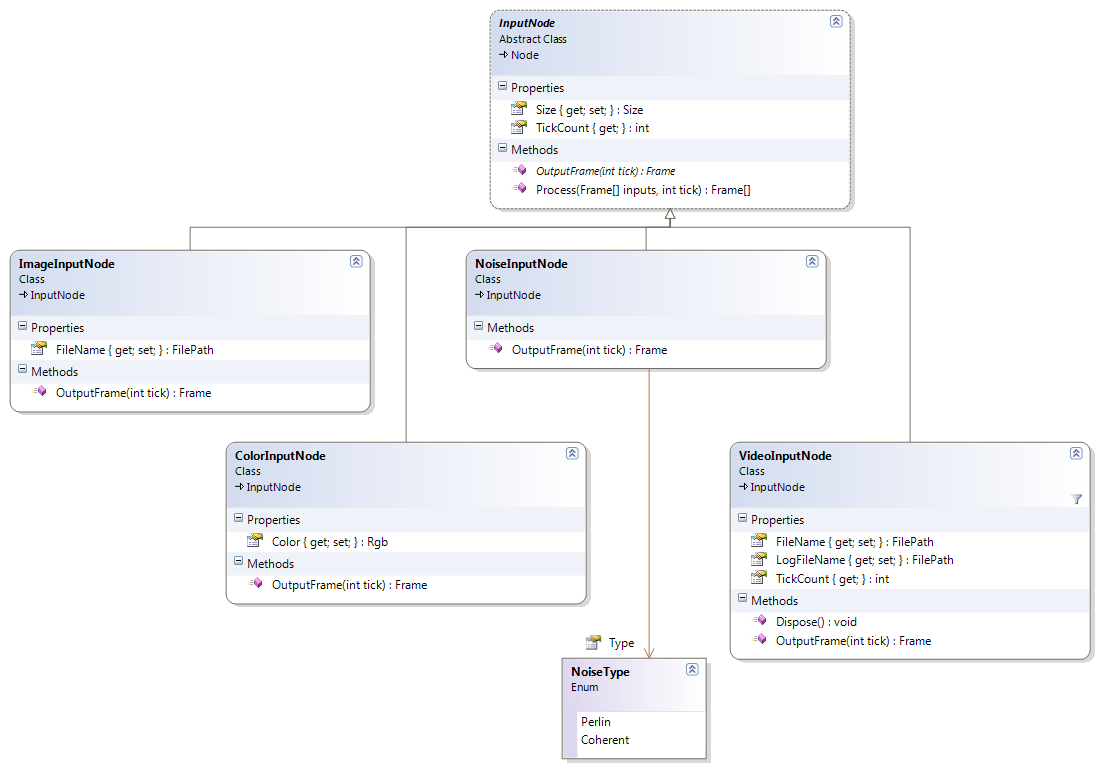
\includegraphics[width=\textwidth]{YuvKA.Pipeline/inputnodes.png}
Der im Folgenden spezifizierte Teil des Programmes beschreibt die Knoten, welche die Eingabedaten der Pipeline bereitstellen. Alle solchen Knoten erben von der abstrakten Klasse \name{InputNode}, welche die Member \name{TickCount} und \name{Size} definiert, die die Anzahl an zu liefernden \name{Frame}s bzw. die Größe eines jeden \name{Frame}s angeben.
\name{InputNode} selbst erbt von der \name{Node}-Klasse.


\subsubsection{YuvKA.Pipeline.InputNode}

\begin{verbatim}
[DataContract]
public abstract class InputNode : Node
\end{verbatim}

\paragraph{Beschreibung}~\\
Die abstrakte Klasse \name{InputNode} modelliert die Eingabequellen der Pipeline und liefert eine gemeinsame Basis für deren konkrete Implementierungen.

\paragraph{Typmember}
\begin{itemize}

\property{Size}
	\begin{verbatim}
	[DataMember]
	public Size Size { get; set; }
	\end{verbatim}
	Spezifiziert die Größe des vom Knoten gelieferten \name{Frame}s in Form eines \name{Size}-Objektes.

\property{TickCount}
	\begin{verbatim}
	[Browsable(false)]
	public virtual int TickCount { get; }
	\end{verbatim}
	Ruft die Anzahl an vom Knoten zu liefernden \name{Frame}s ab. Der Standardrückgabewert ist 1, die Methode ist allerdings in Unterklassen überschreibbar.

\end{itemize}

\subsubsection{YuvKA.Pipeline.ImageInputNode}

\begin{verbatim}
[DataContract]
public class ImageInputNode : InputNode
\end{verbatim}

\paragraph{Beschreibung}~\\
Die Klasse \name{ImageInputNode} stellt die Funktionalität eines Knotens dar, der lediglich ein aus einer Datei im PNG-Format gelesenes Standbild in die Pipeline einspeist. Sie erbt von der abstrakten \name{InputNode}-Klasse.

\paragraph{Typmember}
\begin{itemize}

\property{FileName}
	\begin{verbatim}
[DisplayName("File Name")]
[DataMember]
public FilePath FileName { get; set; }
	\end{verbatim}
	Entspricht dem Dateipfad der zu benutzenden Datei.

\method{Process}
	\begin{verbatim}
	public override Frame[] Process(Frame[] inputs, int tick)
	\end{verbatim}
	Ignoriert den Wert der Eingabeparameter und liefert als Rückgabewert ein Array der Größe 1, das einen \name{Frame} mit den Bilddaten der Datei (aus dem Pfad \name{FileName}) enthält.

\end{itemize}
\subsubsection{YuvKA.Pipeline.ColorInputNode}

\begin{verbatim}
[DataContract]
public class ColorInputNode : InputNode
\end{verbatim}

\paragraph{Beschreibung}~\\
Die Klasse \name{ColorInputNode} liefert die Funktionalität, einen Videostream einer benutzerdefinierten Farbe in Form von \name{Frame}s an die Pipeline zu liefern. Sie erbt von der abstrakten \name{InputNode}-Klasse.

\paragraph{Typmember}
\begin{itemize}

\property{Color}
	\begin{verbatim}
	[DataMember]
	public Rgb Color { get; set; }
	\end{verbatim}
	Entspricht der als Quellwert benutzten Farbe.


\method{Process}
	\begin{verbatim}
	public override Frame[] Process(Frame[] inputs, int tick)
	\end{verbatim}
	Ignoriert den Wert der Eingabeparameter und liefert als Rückgabewert ein Array der Größe 1, das einen \name{Frame} enthält welcher vollends mit der vom Benutzer gewählten Farbe ausgefüllt ist.

\end{itemize}

\subsubsection{YuvKA.Pipeline.NoiseInputNode}

\begin{verbatim}
[DataContract]
public class NoiseInputNode : InputNode
\end{verbatim}

\paragraph{Beschreibung}~\\
Die Klasse \name{NoiseInputNode} stellt einen Knoten bereit, welcher eine von zwei Arten zufällig generierter Videostreams in Form von \name{Frame}s mit Rauschsignal an die Pipeline liefert. Die Klasse erbt von der abstrakten \name{InputNode}-Klasse.

\paragraph{Typmember}
\begin{itemize}

\property{Type}
	\begin{verbatim}
	[DataMember]
	public NoiseType Type { get; set; }
	\end{verbatim}
	Setzt den Typ des Videostreams fest, welcher generiert wird. Standardmäßig werden folgende Verfahren unterstützt:
	\begin{description}
		\item[Perlin-Noise]~\\
		Bei Perlin-Noise werden pseudozufällige Signale dadurch generiert, dass die Koordinaten des angefragten Punktes anhand eines vorgerechneten Rasters mit zufälligen Vektoren nachgeschlagen werden. Der resultierende Wert ist das Resultat des Skalarproduktes aus Abstandsvektors (zum nächsten Rasterpunkt) mit dem im Raster gefundenen Vektor, kombiniert mit einfacher Interpolation, um das resultierende Bild stetig zu halten. PseudoCode der 2-dimensionalen Version:
\begin{verbatim}
public double PerlinNoise(int x, int y) {
  int xint = Math.floor(x);
  int yint = Math.floor(y);
  // Vorberechnete Vektoren an nächsten Gitterpunkten
  // nachschlagen und das Skalarprodukt mit dem 
  // Abstandsvektor zu den Koordinaten bilden
  latticeVect0 = DotProduct(randVectors[xint, yint],
                            (x - xint, y - yint) );
  latticeVect1 = DotProduct(randVectors[xint+1, yint], 
                            (x - xint-1, y - yint) );
  latticeVect2 = DotProduct(randVectors[xint, yint+1], 
                            (x - xint, y - yint-1) );
  latticeVect3 = DotProduct(randVectors[xint+1, yint+1], 
                            (x - xint-1, y - yint-1) );

  // Resultate interpolieren
  xValue = interpolate(latticeVect0, latticeVect1);
  yValue = interpolate(latticeVect2, latticeVect3);
  return interpolate(xValue, yValue);
\end{verbatim}
        Das Resultat von diesem Algorithmus muss bei der weiteren Verarbeitung noch an den Farbraum (hier RGB) angepasst werden. Anzumerken ist, dass es sich hierbei um die ``Rohform'' des Algorithmus handelt, bei der nur eine Iteration durchgeführt wird.
		\item[Coherent Noise]~\\
		Hierbei handelt es sich um einfaches, kohärentes Bildrauschen, welches pixelweise erzeugt wird.
	\end{description}

\method{Process}
	\begin{verbatim}
	public override Frame[] Process(Frame[] inputs, int tick)
	\end{verbatim}
	Ignoriert den Wert der Eingabeparameter und liefert als Rückgabewert ein Array der Größe 1, das den generierten \name{Frame} enthält. Das benutzte Generierungsverfahren hängt vom Wert von \name{Type} ab.


\end{itemize}

\subsubsection{YuvKA.Pipeline.VideoInputNode}

\begin{verbatim}
[DataContract]
public class VideoInputNode : InputNode
\end{verbatim}

\paragraph{Beschreibung}~\\
Die Klasse \name{VideoInputNode} modelliert einen Knoten, welcher die Daten eines aus einer Datei gelesenen Videostream in die Pipeline einspeist. Befindet sich an der durch \name{LogFileName} angegebenen Stelle eine gültige Log-Datei, so wird diese als Metadaten mit einem \name{AnnotatedFrame} mitgereicht. Sie erbt von der abstrakten \name{InputNode}-Klasse.


\paragraph{Typmember}
\begin{itemize}

\property{FileName}
        \begin{verbatim}
[DisplayName("Video File")]
[DataMember]
public FilePath FileName { get; set; }
        \end{verbatim}
	Ruft den Dateipfad der zu lesenden Videodatei ab oder setzt diesen fest.

\property{LogFileName}
        \begin{verbatim}
[DisplayName("Optional Log File")]
[DataMember]
public FilePath LogFileName { get; set; }
        \end{verbatim}
	Ruft den Dateipfad der (optionalen) zu lesenden Log-Datei ab oder setzt diesen fest.

\property{TickCount}
        \begin{verbatim}
[Browsable(false)]
public override int TickCount { get; }
        \end{verbatim}
	Ruft die Anzahl der im Videostream befindlichen \name{Frame}s ab.

\method{Dispose}
        \begin{verbatim}
public override void Dispose()
        \end{verbatim}
Schließt den Videostream, sodass das File-Handle freigegeben wird.


\end{itemize}

\subsection{Manipulationsknoten}

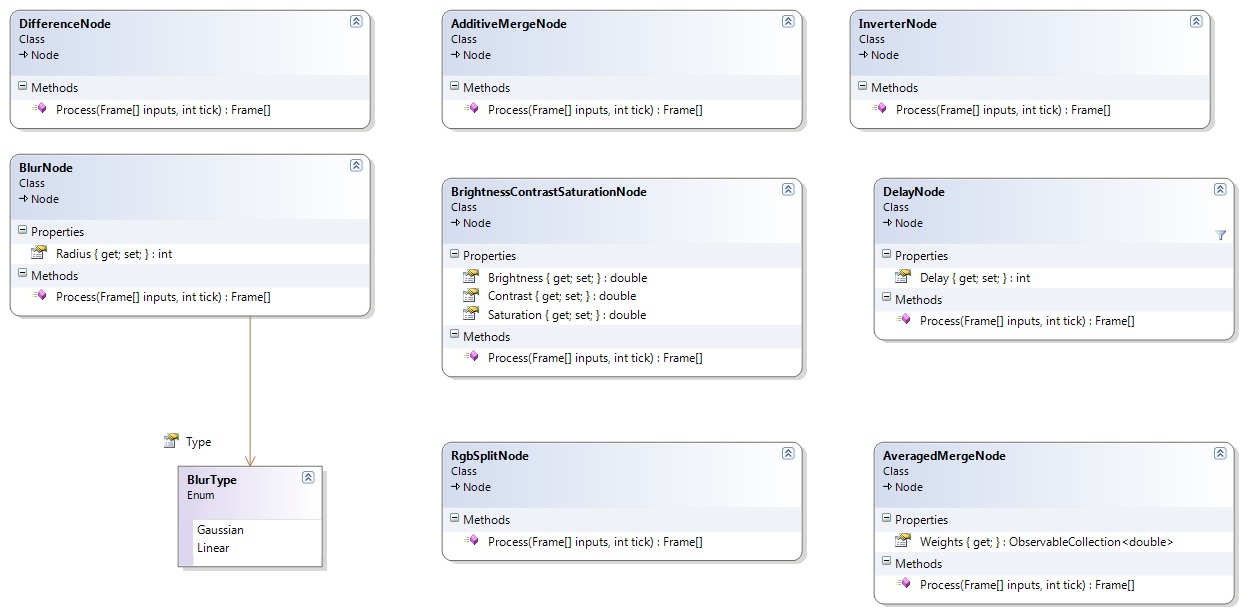
\includegraphics[width=\textwidth]{YuvKA.Pipeline/manipulationnodes.png}
Diese Klassen sind für die Manipulation der Videos innerhalb der Pipeline zuständig. Die einzelnen Knoten sowie deren Implementation werden im Folgenden erläutert. All diese Knoten erben von der abstrakten Klasse \name{Node}.

\subsubsection{YuvKA.Pipeline.InverterNode}
\begin{verbatim}
public class InverterNode : Node
\end{verbatim}

\paragraph{Beschreibung}~\\
Die Klasse \name{InverterNode} invertiert die Farben des \name{Frame}s.

\paragraph{Typmember}
\begin{itemize}

\method{ProcessFrame}
	\begin{verbatim}
	public override Frame[] ProcessFrame(Frame[] inputs, int tick)
	\end{verbatim}
	Invertiert die Farbe der einzelnen Pixel des \name{Frame}s. Dafür wird das Komplement von jedem der drei Farbkanäle eines Pixels gebildet.

\end{itemize}


\subsubsection{YuvKA.Pipeline.BlurNode}

\begin{verbatim}
[DataContract]
public class BlurNode : Node
\end{verbatim}

\paragraph{Beschreibung}~\\
Die Klasse \name{BlurNode} modelliert die Weichzeichnung der \name{Frame}s des Videos.

\paragraph{Typmember}
\begin{itemize}

\property{Type}
	\begin{verbatim}
	[DataMember]
	public BlurType Type { get; set; }
	\end{verbatim}
	Ruft die Art der Weichzeichnung ab oder legt sie fest. Standardmäßig werden gaußsches und lineares Weichzeichnen unterstützt.
	
\property{Radius}
	\begin{verbatim}
	[DataMember]
	[Range(0.0, double.PositiveInfinity)]
	public int Radius { get; set; }
	\end{verbatim}
	Ruft den Weichzeichnungsradius ab oder legt diesen fest. Dieser Wert ist maßgeblich für das Ausmaß der Weichzeichnung.

\method{ProcessFrame}
	\begin{verbatim}
	public override Frame[] ProcessFrame(Frame[] inputs, int tick)
	\end{verbatim}
	Zeichnet den übergebenen \name{Frame} weich. Die genaue Art der Weichzeichnung wird hierbei durch \name{Type} festgelegt. Die standardmäßig unterstützten Arten sind:
	\begin{description}
		\item[Lineares Weichzeichnen]~\\
			Beim linearen Weichzeichnen wird der neue Wert eines Pixels dadurch berechnet, dass die alten Werte aller umliegenden Pixel innerhalb einer Box mit Höhe und Breite (2 * \name{Radius}) + 1 gemittelt werden. Über den \name{Frame}rand hinaus benötigte Pixel werden durch den Pixel, der dem gesuchten Pixel am nächsten ist, simuliert. ~\\~\\
			PseudoCode:
			\begin{verbatim}
				Frame newFrame = new Frame(inputs[0])
				for (int x = 0; x < inputs[0].Size.X; x++)
				  for (int y = 0; y < inputs[0].Size.Y; y++)
				    newFrame(x, y) = 0
				    for (xi = x - Radius; xi <= x + Radius; xi++)
				      for (yi = y - Radius; yi <= y + Radius; yi++)
				        newFrame(x, y) += (1 / (Radius * Radius))
				                           * inputs[0](x, y)
				return newFrame
				
			\end{verbatim}
		\item[Gaußsches Weichzeichnen]~\\
			Beim Gaußschen Weichzeichnen wird der neue Wert eines Pixels durch eine gewichtete Mittelung der umliegenden Pixel berechnet. Die Gewichtung der umliegenden Pixel wird hierbei durch folgende gaußsche Funktion definiert:\\
			\[
			G(x,y) = \frac{1}{\sqrt{2\pi\sigma^2}}e^{-\frac{x^2}{2\sigma^2}}
			\]
			Wobei $\sigma$ der \name{Radius} ist.\\
			 Über den \name{Frame}rand hinaus benötigte Pixel werden durch den Pixel, der dem gesuchten Pixel am nächsten ist, simuliert.~\\~\\
			PseudoCode:
			\begin{verbatim}
				Frame newFrame = new Frame(inputs[0])
				for (int x = 0, x < inputs[0].size.x, x++)
				  for (int y = 0, y < inputs[0].size.y, y++)
				    newFrame.Data[x][y] = 0
				    for (int xi = x - (3 * Radius); xi < x + (3 * Radius;, xi++)
				      for (int yi = y - (3 * Radius); yi < y + (3 * Radius); yi++)
				        newFrame.Data[x][y] += G(xi - x, yi - y) * inputs[0].Data[x][y]
				return newFrame
				
			\end{verbatim}
	\end{description}
	
\end{itemize}


\subsubsection{YuvKA.Pipeline.BrightnessContrastSaturationNode}

\begin{verbatim}
[DataContract]
public class BrightnessContrastSaturationNode : Node
\end{verbatim}

\paragraph{Beschreibung}~\\
Diese Klasse \name{BrightnessContrastSaturationNode} ändert die Helligkeit, den Kontrast und/oder die Farbsättigung des \name{Frame}s.

\begin{itemize}

\property{Brightness}
	\begin{verbatim}
	[DataMember]
	[Range(-1.0, 1.0)]
	public double Brightness
	\end{verbatim}
	Ruft den Helligkeitswert, zu dem dieses \name{Frame} gesetzt werden soll, ab oder legt ihn fest. Der Wert muss zwischen -1.0 und 1.0 liegen.
	
\property{Contrast}
	\begin{verbatim}
	[DataMember]
	[Range(-1.0, 1.0)]
	public double Contrast
	\end{verbatim}
	Ruft den Kontrastwert, zu dem dieses \name{Frame} gesetzt werden soll, ab oder legt ihn fest. Der Wert muss zwischen -1.0 und 1.0 liegen.
	
\property{Saturation}
	\begin{verbatim}
	[DataMember]
	[Range(-1.0, 1.0)]
	public double Saturation
	\end{verbatim}
	Ruft den Farbsättigungswert, zu dem dieses \name{Frame} gesetzt werden soll, ab oder legt ihn fest. Der Wert muss zwischen -1.0 und 1.0 liegen.

\method{ProcessFrame}
	\begin{verbatim}
	public override Frame[] ProcessFrame(Frame[] inputs, int tick)
	\end{verbatim}
	Die Methode \name{ProcessFrame} setzt die Helligkeit, den Kontrast und die Farbsättigung des \name{Frame}s auf die gegebenen Werte. Dafür werden die Farbkanäle jedes Pixels aus dem RGB-Raum in den HSL-Raum umgerechnet, die Änderungen vorgenommen und anschließend wieder nach RGB konvertiert. Für die RGB - HSL Konvertierung werden die Methoden \name{Color.GetHue}, \name{Color.GetSaturation} und \name{Color.GetBrightness} aus dem .NET Framework benutzt. Für die Rückrichtung wird folgender Algorithmus benutzt:
	\floatname{algorithm}{Algorithmus}
	\begin{algorithm}[H]
	\caption{HSL nach RGB Konvertierung}
		\begin{algorithmic}[1]
			\REQUIRE $ H \in [0^\circ, 360^\circ], \ S \in [0, 1], \ L \in [0, 1] $ \\
			\COMMENT {Als erstes berechnen wir die Chroma. Dann können wir einen Punkt $ (R_1, G_1, B_1) $ mit dem gleichen Farbton und Chroma wie unsere Farbe entlang der unteren drei Seiten des RGB-Würfels finden, indem wir einen temporären Wert $ X $ für ihre zweitgrößte Komponente benutzten.}
			\vspace{3px}
			\STATE $ C \gets (1 - |2L - 1|) \cdot S $
			\STATE $ H' = \frac{H}{60^\circ} $
			\STATE $ X = C(1 - |H' \ mod \ 2 - 1|) $
			\vspace{3px}
			\STATE $ (R_1, G_1, B_1) \gets
					\begin{cases} 
						(0, 0, 0), & \text{falls } S = 0 \\
						(C, X, 0), & \text{falls } 0 \leq H' < 1 \\
						(X, C, 0), & \text{falls } 1 \leq H' < 2 \\
						(0, C, X), & \text{falls } 2 \leq H' < 3 \\
						(0, X, C), & \text{falls } 3 \leq H' < 4 \\
						(X, 0, C), & \text{falls } 4 \leq H' < 5 \\
						(C, 0, X), & \text{falls } 5 \leq H' < 6 \\
					\end{cases}
				   $
			\vspace{3px} \\
			\COMMENT { Schließlich erhalten wir R, G, und B durch das dazuaddieren des gleichen Werts, damit sie mit der Helligkeit übereinstimmen.}
			\vspace{3px}
			\STATE $ m \gets L - \frac{1}{2}C $
			\STATE $ (R, G, B) \gets (R_1 + m, G_1 + m, B_1 + m) $
			\vspace{3px}
			\ENSURE $ R, \ G, \ B \in [0, 1] $ \\
			\COMMENT {Ist $ S = 0$ , dann ist die resultierende Farbe Neutralgrau, und die Formel vereinfacht sich zu $ R = G = B = L $.}
		\end{algorithmic}
	\end{algorithm}
	
	Nach der RGB - HSV Konvertierung können die S (Sättigung) und V (Helligkeit) Werte in den oben angegebenen Schranken modifiziert werden, um dann wieder nach RGB umgewandelt zu werden und in den neuen Pixeln geschrieben zu werden. \\
	Für den Kontrast ist lediglich der Abstand zwischen einem Farbkanal und 128 zu vergrößern, wie in der folgenden Formel zu sehen ist: \begin{eqnarray*}
   r = (r - 128) \cdot \text{\name{Contrast}} + 128 \\
	g = (g - 128) \cdot \text{\name{Contrast}} + 128 \\
	b = (b - 128) \cdot \text{\name{Contrast}} + 128
\end{eqnarray*}

\end{itemize}

\subsubsection{YuvKA.Pipeline.AdditiveMergeNode}

\begin{verbatim}
public class AdditiveMergeNode : Node
\end{verbatim}

\paragraph{Beschreibung}~\\
Diese Klasse \name{AdditiveMergeNode} legt mehrere Frames additiv übereinander.

\begin{itemize}

\method{ProcessFrame}
\begin{verbatim}
	public override Frame[] ProcessFrame(Frame[] inputs, int tick)
\end{verbatim}
Die Methode \name{ProcessFrame} legt mehrere Frames additiv übereinander, indem sie die Farbwerte der positionsgleichen Pixel addiert und den so entstandenen Farbwert als das neue Pixel speichert.
\end{itemize}

\subsubsection{YuvKA.Pipeline.AveragedMergeNode}

\begin{verbatim}
[DataContract]
public class AveragedMergeNode : Node
\end{verbatim}

\paragraph{Beschreibung}~\\
Die Klasse \name{AveragedMergeNode} modelliert das Zusammenführen von Videos durch gewichtete Mittelung der \name{Frame}s.

\paragraph{Typmember}
\begin{itemize}

\property{Weights}
	\begin{verbatim}
		[DataMember]
		[Range(0.0, 1.0)]
		public ObservableCollection<double> Weights { get; }
	\end{verbatim}
	Ruft eine Sammlung von Gewichtungen einzelner Videos ab.

\method{ProcessFrame}
	\begin{verbatim}
	public override Frame[] ProcessFrame(Frame[] inputs, int tick)
	\end{verbatim}
	Mittelt alle übergebenen \name{Frame}s Pixelweise unter Beachtung der von \name{Weights} definierten Gewichtungen. Falls zwei Videos mit verschiedener Auflösung zusammengeführt werden, so wird das Maximum der Höhe bzw. Breite der beiden Videos als Auflösung des neuen Videos genommen. Fehlende Bildinformationen bei auflösungstechnisch kleineren Videos werden durch Schwarz ergänzt.\\~\\
	PseudoCode:
	\begin{verbatim}
		Frame newFrame = new Frame(inputs[0])
		for (int x = 0; x < inputs[0].Size.X; x++)
		  for (int y = 0; y < inputs[0].Size.Y; y++)
		    newFrame(x, y) = 0
		    int sumOfWeights = 0
		    for (int i = 0; i < inputs.Size(); i++)
		      newFrame(x, y) += inputs[i](x, y) * Weights[i]
		      sumOfWeights += Weights[i]
		    newFrame(x, y) = newFrame(x, y) / sumOfWeights
		return newFrame
		
	\end{verbatim}
	
\end{itemize}

\subsubsection{YuvKA.Pipeline.DifferenceNode}

\begin{verbatim}
public class DifferenceNode : Node
\end{verbatim}

\paragraph{Beschreibung}~\\
Die Klasse \name{DifferenceNode} bildet die Differenz zweier \name{Frame}s.

\begin{itemize}
\method{ProcessFrame}
	\begin{verbatim}
		public override Frame[] ProcessFrame(Frame[] inputs, int tick)
	\end{verbatim}
Die Methode \name{ProcessFrame} bildet die Differenz zweier \name{Frame}s, indem sie die Farbwerte positionsgleicher Pixel subtrahiert.

\end{itemize}

\subsubsection{YuvKA.Pipeline.DelayNode}

\begin{verbatim}
[DataContract]
public class DelayNode : Node
\end{verbatim}

\paragraph{Beschreibung}~\\
Die Klasse \name{DelayNode} modelliert die Verzögerung von Videostreams innerhalb der Pipeline.

\paragraph{Typmember}
\begin{itemize}
	
\property{Delay}
	\begin{verbatim}
	[DataMember]
	[Range(0, 10)]
	public int Delay { get; set; }
	\end{verbatim}
	Ruft die Dauer der Verzögerung in der Einheit \name{Frame}s ab oder legt sie fest.

\method{ProcessFrame}
	\begin{verbatim}
	public override Frame[] ProcessFrame(Frame[] inputs, int tick)
	\end{verbatim}
	Stellt den übergebenen \name{Frame} in eine Warteschlange mit der Länge \name{Delay} an, und gibt den ersten \name{Frame} der Warteschlange zurück.
	
\end{itemize}

\subsubsection{YuvKA.Pipeline.RgbSplitNode}

\begin{verbatim}
public class RgbSplitNode : Node
\end{verbatim}

\paragraph{Beschreibung}~\\
Die Klasse \name{RgbSplitNode} modelliert die Aufteilung der \name{Frame}s eines Videos in die Farbkanäle Rot, Grün und Blau.

\paragraph{Typmember}
\begin{itemize}

\method{ProcessFrame}
	\begin{verbatim}
	public override Frame[] ProcessFrame(Frame[] inputs, int tick)
	\end{verbatim}
	Erzeugt aus dem übergebenen \name{Frame} drei neue \name{Frame}s die jeweils nur einen Farbkanal des ursprünglichen \name{Frame}s enthalten und gibt diese zurück.
	
\end{itemize}

\subsection{Ausgabeknoten}

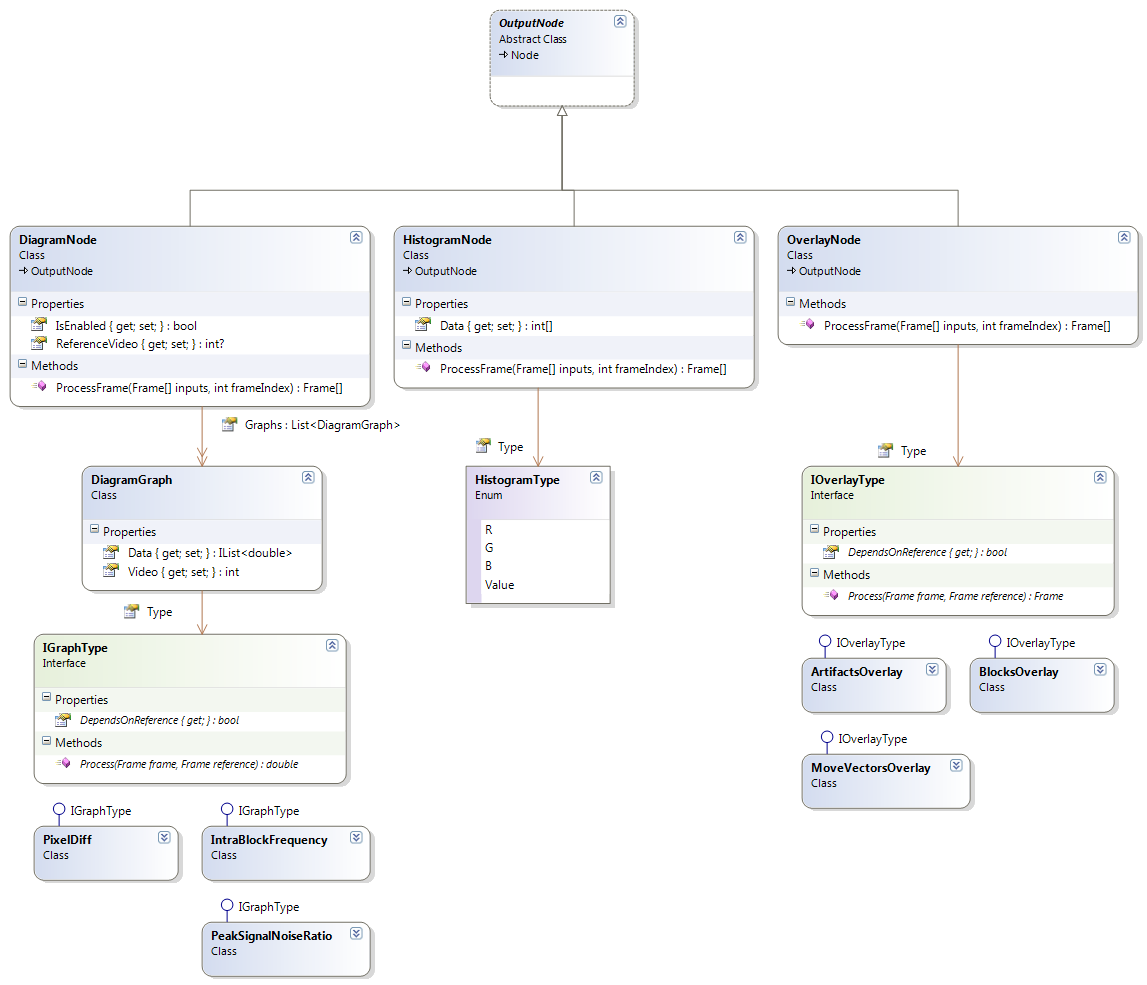
\includegraphics[width=\textwidth]{YuvKA.Pipeline/outputnodes.png}
Die folgenden Klassen stellen Knoten zur Verfügung, die die Ausgabe und Analyse der Videos der Pipeline übernehmen. All diese Klassen erben von der abstrakten Klasse \name{OutputNode}, welche wiederum von der abstrakten Klasse \name{Node} erbt.

\subsubsection{YuvKA.Pipeline.OutputNode}

\begin{verbatim}
public abstract class OutputNode : Node
\end{verbatim}

\paragraph{Beschreibung}~\\
Die abstrakte Klasse \name{OutputNode} modelliert die Ausgabemöglichkeiten der Pipeline und bietet eine gemeinsame Basis für deren konkrete Implementationen.

\subsubsection{YuvKA.Pipeline.DiagramNode}

\subsubsection{YuvKA.Pipeline.HistogramNode}

\begin{verbatim}
public class HistogramNode : OutputNode
\end{verbatim}
Die Klasse \name{HistogramNode} stellt die Daten zur Verfügung, die von dem \name{HistogramViewModel} verwendet werden, um die Histogrammgrafiken darzustellen. Es werden für jeden der drei Farbkanäle sowie für für den Farbwert V im HSV-Raum jeweils ein Histogramm unterstützt.

\paragraph{Typmember}
\begin{itemize}
\property{Type}
	\begin{verbatim}
		[Browsable(false)]
		public HistogramType Type
	\end{verbatim}
	Ruft den Histogrammtyp ab oder legt ihn fest. Es werden vier Arten von Histogrammen unterstützt: jeweils einen für jeden der drei Farbkanäle, sowie einen für den Farbwert im HSV-Raum.
	
\property{Data}
	\begin{verbatim}
		[Browsable(false)]
		public double[] Data { get; private set; }
	\end{verbatim}
	Ruft ein Array der Größe 256 ab, in dem die Verteilung des Farbkanals oder HSV-Farbwerts im \name{Frame} dargestellt ist. Die Stelle $ i \ (0 \leq i \leq 255) $ im Array speichert die Häufigkeit des Farbwerts $ i $ im \name{Frame} für den gewählten Farb\name{typ} (R, G, B oder V). Der Wert liegt zwischen 0.0 und 1.0, da eine relative Häufigkeit dargestellt wird.

\method{ProcessFrame}
	\begin{verbatim}
		public override Frame[] ProcessFrame(Frame[] inputs, int frameIndex)
	\end{verbatim}
	Die Methode \name{ProcessFrame} berechnet für den angegebenen Histogramm\name{typ} die Häufigkeit der Farbwerte von 0 bis 255 und speichert diese an der entsprechenden Stelle im Array \name{Data}, wie im folgenden Algorithmus zu sehen ist:
	\floatname{algorithm}{Algorithmus}
	\begin{algorithm}[H]
		\caption{Berechnung der relativen Häufigkeit eines Farbtyps}
		\begin{algorithmic}[1]
			\REQUIRE $ PIXELS, $ \COMMENT { Die Menge aller Pixel im Frame.}
			\STATE \COMMENT{ Sei $ f_{t}(p) $ der Wert der Farbe $ t $ im Pixel $ p \ (t \in \{ R, G, B, V \})$, $ t $ festgesetzt in \name{Type}. \\ $ D_i $ entspricht dem \textbf{Data} Array.}
			\FORALL{$ p \in PIXELS $}
				\STATE $ i \gets f_{t}(p) $
				\STATE $ D_i \gets D_i + 1 $
			\ENDFOR
			\FOR{$ i \gets 0 \text{\textbf{ to }} 255 $}
				\STATE $ D_i \gets \frac{D_i}{|PIXELS|} $
			\ENDFOR
			\ENSURE $ D_i, $ \COMMENT { Das Ausgabearray, in dem die Verteilung gespeichert ist.}
		\end{algorithmic}
	\end{algorithm}

\end{itemize}

\subsubsection{YuvKA.Pipeline.OverlayNode}

\begin{verbatim}
[DataContract]
public class OverlayNode : OutputNode
\end{verbatim}

\paragraph{Beschreibung}~\\
Die Klasse \name{OverlayNode} modelliert das überlagern von Videos mit graphischen Darstellungen von Analysedaten.

\paragraph{Typmember}
\begin{itemize}

\property{Type}
	\begin{verbatim}
	[DataMember]
	public IOverlayType Type { get; set; }
	\end{verbatim}
	Ruft die Art der Überlagerung ab, oder legt sie fest. Standardmäßig werden die Markierung von Artefakten im Vergleich mit einem Referenzvideo, das Anzeigen von Bewegungsvektoren sowie eine Anzeige der Makroblockentscheidungen des Encoders unterstützt.

\method{ProcessFrame}
	\begin{verbatim}
	public override Frame[] ProcessFrame(Frame[] inputs, int frameIndex)
	\end{verbatim}
	Überlagert den übergebenen \name{Frame} mit den durch \name{Type} spezifizierten Daten und gibt den Überlagerten \name{Frame} zurück. Bei den standardmäßig unterstützen Möglichkeiten handelt es sich um:
	\begin{description}
		\item[Artefaktüberlagerung]~\\
			Für diese Überlagerung werden zwei Eingabeframes benötigt, da hier die Artefakte eines \name{Frame}s im Vergleich mit einem anderen hervorgehoben werden.
		\item[Blocküberlagerung]~\\
			Für diese Überlagerung wird eine Eingabe in Form eines \name{AnnotatedFrame}s benötigt, da aus den Logdateien die Makroblockentscheidungen des Encoders entnommen werden. Diese werden durch durch Einzeichnen der vom Encoder eingeteilten Inter- und Intramakroblöcken in die übergebene \name{Frame} dargestellt.
		\item[MoveVectorsOverlay]~\\
			Für diese Überlagerung wird eine Eingabe in Form eines \name{AnnotatedFrame}s benötigt, da aus den Logdateien die erkannten Bewegungsvektoren des Encoders entnommen werden um diese in den \name{Frame} einzuzeichnen.
	\end{description}
	
\end{itemize}

\section{YuvKA.ViewModel}
\subsection{Hauptoberfläche}

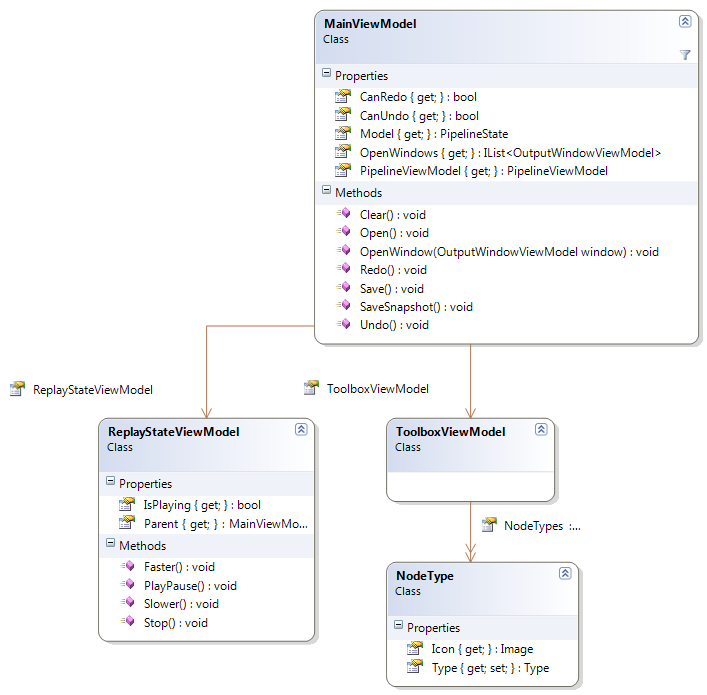
\includegraphics[width=\textwidth]{YuvKA.ViewModel/main.png}
Das Programm wird durch Instanzierung des \name{MainViewModel}s und Anzeigen der zugehörigen View gestartet. Diese Klasse delegiert Einheiten der Hauptoberfläche an untergeordnete View Models, wobei die Klassen zur Anzeige des Pipeline-Graphen erst im nächsten Abschnitt beschrieben werden.

\subsubsection{MainViewModel}

\begin{verbatim}
public class MainViewModel
\end{verbatim}

\paragraph{Beschreibung}~\\
Die \name{MainViewModel}-Klasse hält das Programm-Model in Form einer \name{PipelineState}-Instanz, verwaltet es in einem Undo/Redo-System und instanziert weitere untergeordnete View Models.

\paragraph{Typmember}
\begin{itemize}

\property{CanUndo, CanRedo}
	\begin{verbatim}
	public bool CanUndo { get; }
	public bool CanRedo { get; }
	\end{verbatim}
	Ruft ab, ob ein Rückgängig- bzw. Wiederholen-Schritt zur Verfügung steht.

\property{Model}
	\INPC
	\begin{verbatim}
	public PipelineState Model { get; }
	\end{verbatim}
	Stellt das derzeitige Model-Objekt für Data Binding und untergeordnete View Models zur Verfügung.

\property{OpenWindows}
	\begin{verbatim}
	public IList<OutputWindowViewModel> OpenWindows { get; }
	\end{verbatim}
	Ruft eine Liste der derzeit geöffneten Ausgabefenster ab.

\property{ReplayStateViewModel, PipelineViewModel, ToolboxViewModel}
	Ruft jeweils eine Instanz der gleichnamigen Klasse ab.

\method{Clear, Open}
	\begin{verbatim}
	public void Clear()
	public void Open()
	\end{verbatim}
	Ersetzen das derzeitige Model durch eine neue leere bzw. aus einer Datei geladenen Pipeline, dabei wird jeweils ein neuer Rückgangig-Schritt erzeugt. Open öffnet zusätzlich einen \name{OpenFileDialog} zur Auswahl des Dateipfades.

\method{Save}
	\begin{verbatim}
	public void Save()
	\end{verbatim}
	Speichert das derzeitige Model in einer Datei ab. Dazu öffnet Save einen \name{SaveFileDialog} und serialisiert dann das \name{Model}-Objekt in die gewählte Datei.

\method{SaveSnapshot()}
	\begin{verbatim}
	public void SaveSnapshot()
	\end{verbatim}
	Hält den aktuellen Model-Zustand als Rückgängig-Schritt fest. Alle Wiederholen-Schritte werden verworfen.

\method{Undo, Redo}
	\begin{verbatim}
	public void Undo()
	public void Redo()
	\end{verbatim}
	Stellt den Zustand des nächsten Rückgängig- bzw. Wiederholen-Schrittes wieder her.

\end{itemize}
\subsection{Pipeline-Graph}

\begin{center}	
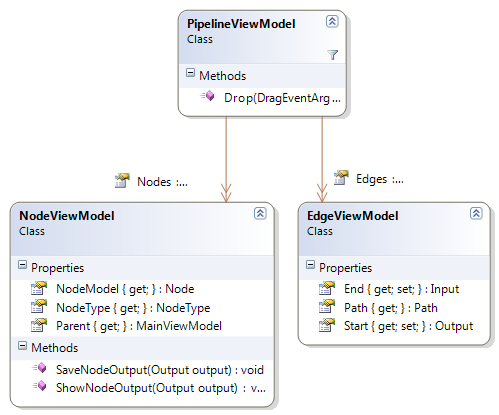
\includegraphics[width=0.5\textwidth]{YuvKA.ViewModel/pipeline.png}
\end{center}
Die Klasse \name{PipelineViewModel} und ihre untergeordneten ViewModels sind für die Darstellung und Manipulation des Pipeline-Graphen zuständig.

\subsubsection{YuvKA.ViewModel.PipelineViewModel}

\begin{verbatim}
public class PipelineViewModel
\end{verbatim}

\paragraph{Beschreibung}~\\
Die \name{PipelineViewModel}-Klasse erzeugt aus dem Graphen des Models passende ViewModels für Knoten und Kanten.

\paragraph{Typmember}
\begin{itemize}

\property{Nodes}
	\begin{verbatim}
	public IList<NodeViewModel> Nodes { get; }
	\end{verbatim}
	Ruft die Menge der Knoten-ViewModels ab.

\method{Edges}
	\begin{verbatim}
	public IEnumerable<EdgeViewModel> Edges { get; }
	\end{verbatim}
	Ruft eine Auflistung von Kanten-ViewModels ab. Der Propertywert wird bei Abruf dynamisch aus der Knotenmenge erzeugt.

\end{itemize}

\subsubsection{YuvKA.ViewModel.NodeViewModel}

\begin{verbatim}
public class NodeViewModel
\end{verbatim}

\paragraph{Beschreibung}~\\
Die \name{NodeViewModel}-Klasse präsentiert die Daten eines \name{Node}-Objekts, sodass sie von der View gebunden werden können.

\paragraph{Typmember}
\begin{itemize}

\property{NodeModel}
	\begin{verbatim}
	public Node NodeModel { get; }
	\end{verbatim}
	Ruft das repräsentierte \name{Node}-Objekt ab.

\property{NodeType}
	\begin{verbatim}
	public NodeType NodeType { get; }
	\end{verbatim}
	Ruft das \name{NodeType}-Objekt ab, das den Typ von \name{NodeModel} repräsentiert.

\method{SaveNodeOutput}
	\begin{verbatim}
	public void SaveNodeOutput(Output output)
	\end{verbatim}
	Rendert das Video des angegebenen Ausgangs und speichert es in einer per \name{SaveFileDialog} ausgewählten Datei.

\method{ShowNodeOutput}
	\begin{verbatim}
	public void ShowNodeOutput(Output output)
	\end{verbatim}
	Öffnet für den angegebenen Ausgang ein neues \name{VideoOutputViewModel}.

\end{itemize}

\subsubsection{YuvKA.ViewModel.EdgeViewModel}

\begin{verbatim}
public class EdgeViewModel
\end{verbatim}

\paragraph{Beschreibung}~\\
Die \name{EdgeViewModel}-Klasse repräsentiert eine Kante im Pipeline-Graph.

\paragraph{Typmember}
\begin{itemize}

\property{Start, Stop}
	\begin{verbatim}
	public Node.Output Start { get; }
	public Node.Input Stop { get; }
	\end{verbatim}
	Rufen Beginn und Ende der Kante ab oder legen sie fest.

\property{Path}
	\begin{verbatim}
	public Path Path { get; }
	\end{verbatim}
	Ruft eine Bezierkurve ab, die die Kante darstellt.

\end{itemize}

\subsection{Ausgabefenster}
\begin{center}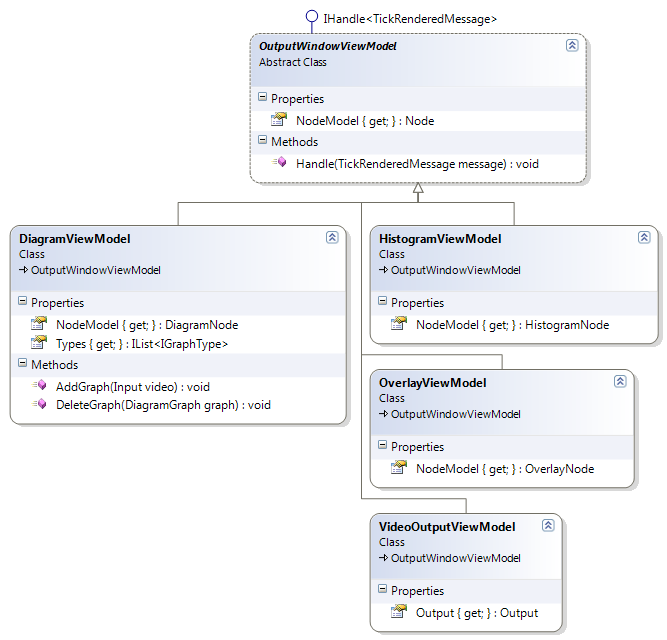
\includegraphics[scale=0.7]{YuvKA.ViewModel/outputs.png} \\
\end{center}
Die abstrakte Klasse \name{OutputWindowViewModel} und ihre konkreten Implementierungen stellen die Daten für die verschiedenen Ausgabefenster, die aus der Hauptoberfläche heraus geöffnet werden können, bereit.

\subsubsection{YuvKA.ViewModel.OutputWindowViewModel}

\begin{verbatim}
public abstract	class OutputWindowViewModel : IHandle<FrameRenderedMessage>
\end{verbatim}

\paragraph{Beschreibung}~\\
Die \name{OutputWindowViewModel}-Klasse hält das \name{Node}-Objekt, das die anzuzeigenden Daten enthält, und reagiert auf \name{FrameRenderedMessage}s, die vom \name{PipelineState} verschickt werden.

\paragraph{Typmember}
\begin{itemize}

\property{NodeModel}
	\begin{verbatim}
public Node NodeModel { get; }
	\end{verbatim}
	\name{Node}-Objekt, das die anzuzeigenden Daten enthält	

\method{Handle}
	\begin{verbatim}
public virtual void Handle(FrameRenderedMessage message)
	\end{verbatim}
	Aktualisiert das Ausgabefenster nach Rendern eines Pipeline-Ticks. Die Standardimplementierung ist leer.

\end{itemize}

\subsubsection{YuvKA.ViewModel.DiagramViewModel}

\begin{verbatim}
public class DiagramViewModel : OutputWindowViewModel
\end{verbatim}

\paragraph{Beschreibung}~\\
Die \name{DiagramViewModel}-Klasse repräsentiert das Ausgabefenster eines \name{DiagramNode}s.

\paragraph{Typmember}
\begin{itemize}

\property{NodeModel}
	\begin{verbatim}
public DiagramNode NodeModel { get; }
	\end{verbatim}
	\name{OutputWindowViewModel.NodeModel}, spezifiziert auf \name{DiagramNode}

\property{Types}
	\begin{verbatim}
public IList<IGraphType> Types { get; }
	\end{verbatim}
	Ermittelt die dynamisch erweiterbare Menge der \name{IGraphType}-Ableitungen und ruft für jede dieser Subklassen eine Instanz ab.

\method{AddGraph}
	\begin{verbatim}
public void AddGraph(Input video)
	\end{verbatim}
	Fügt \name{NodeModel.Graphs} ein neues \name{DiagramGraph}-Objekt mit dem angegebenen Eingabevideo hinzu.

\method{DeleteGraph}
	\begin{verbatim}
public void DeleteGraph(DiagramGraph graph)
	\end{verbatim}
	Löscht den angegebenen Graph aus \name{NodeModel.Graphs}.

%%%%% Interne Klasse Input Hier bitte. %%%%%

\end{itemize}

\subsubsection{YuvKA.ViewModel.HistogramViewModel}

\begin{verbatim}
public class HistogramViewModel : OutputWindowViewModel
\end{verbatim}

\paragraph{Beschreibung}~\\
Die \name{HistogramViewModel}-Klasse repräsentiert das Ausgabefenster eines \name{HistogramNode}s.

\paragraph{Typmember}
\begin{itemize}

\property{NodeModel}
	\begin{verbatim}
public Node NodeModel { get; }
	\end{verbatim}
	\name{OutputWindowViewModel.NodeModel}, spezifiziert auf \name{HistogramNode}

\end{itemize}

\subsubsection{YuvKA.ViewModel.OverlayViewModel}

\begin{verbatim}
public class OverlayViewModel : OutputWindowViewModel
\end{verbatim}

\paragraph{Beschreibung}~\\
Die \name{OverlayViewModel}-Klasse repräsentiert das Ausgabefenster eines \name{OverlayNode}s.

\paragraph{Typmember}
\begin{itemize}

\property{NodeModel}
	\begin{verbatim}
public Node NodeModel { get; }
	\end{verbatim}
	\name{OutputWindowViewModel.NodeModel}, spezifiziert auf \name{OverlayNode}

\end{itemize}

\subsubsection{YuvKA.ViewModel.VideoOutputViewModel}

\begin{verbatim}
public class VideoOutputViewModel : OutputWindowViewModel
\end{verbatim}

\paragraph{Beschreibung}~\\
Die \name{VideoOutputViewModel}-Klasse repräsentiert das Ausgabefenster eines einzelnen Knotenausgangs.

\begin{itemize}

\property{Output}
	\begin{verbatim}
	public Node.Output Output { get; }
	\end{verbatim}
	Ruft den \name{Node.Output} ab, dessen Frameausgabe angezeigt werden soll.

\end{itemize}


\section{YuvKA.ViewModel.PropertyEditor}
\subsection{Property View Models}


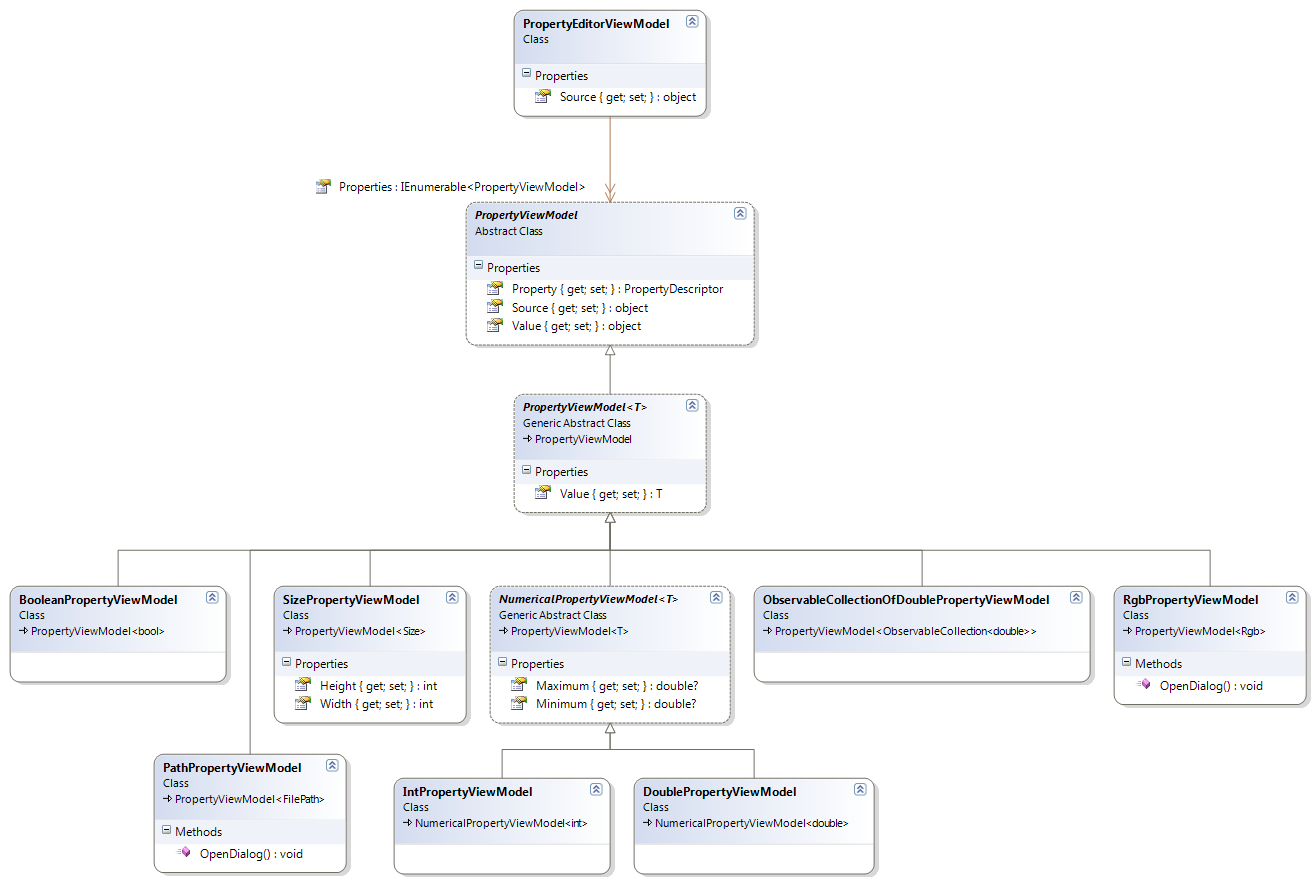
\includegraphics[width=\textwidth]{YuvKA.ViewModel.PropertyEditor/propertyEditor.png}
Diese Klassen dienen der Darstellung der vom Benutzer veränderbaren Properties unter Zuhilfenahme der View. 



\subsubsection{YuvKA.ViewModel.PropertyEditor.PropertyEditorViewModel}

\begin{verbatim}
public class PropertyEditorViewModel
\end{verbatim}

\paragraph{Beschreibung}~\\
Die Klasse \name{PropertyEditorViewModel} verwaltet eine Anzahl von Properties und ermöglicht mithilfe der View ihre Darstellung.

\paragraph{Typmember}
\begin{itemize}

\property{Properties}
	\begin{verbatim}
	public IEnumerable<PropertyViewModel> Properties { get; }
	\end{verbatim}
	Ruft die Liste der zu verwaltenden Properties ab.

\property{Source}
	\begin{verbatim}
	public object Source { get; }
	\end{verbatim}
	Ruft die Quelle der zu verwaltenden Properties ab.

\end{itemize}




\subsubsection{YuvKA.ViewModel.PropertyEditor.PropertyViewModel}

\begin{verbatim}
public abstract class PropertyViewModel
\end{verbatim}

\paragraph{Beschreibung}~\\
Abstrakte Oberklasse zu den einzelnen PropertyViewModel-Klassen

\paragraph{Typmember}
\begin{itemize}
 	
\property{Property}
	\begin{verbatim}
	public PropertyDescriptor Property { get; }
	\end{verbatim}
	Ruft die Beschreibung der verwalteten Property ab.

\property{Source}
	\begin{verbatim}
	public object Source { get; }
	\end{verbatim}
	Ruft die Quelle der verwalteten Property ab.

\property{Value}
	\begin{verbatim}
	public object Value { get; set; }
	\end{verbatim}
	Ruft den Wert der verwalteten Property ab oder legt ihn fest.

\end{itemize}




\subsubsection{YuvKA.ViewModel.PropertyEditor.PropertyViewModel\textless T\textgreater}

\begin{verbatim}
[InheritedExport]
public abstract class PropertyViewModel<T> : PropertyViewModel
\end{verbatim}

\paragraph{Beschreibung}~\\
Typisierte Ableitung der \name{PropertyViewModel}-Klasse

\paragraph{Typmember}
\begin{itemize}

\property{Value}
	\begin{verbatim}
	public T Value { get; set; }
	\end{verbatim}
	Ruft den Wert der Property ab oder legt ihn fest. T ist hierbei der Typ der verwalteten Property.
\end{itemize}



\subsubsection{PropertyViewModel-Implementierungen}

\begin{itemize}

\item{\textbf{YuvKA.ViewModel.PropertyEditor.BooleanPropertyViewModel}}
	\begin{verbatim}
	public class BooleanPropertyViewModel : PropertyViewModel<bool>
	\end{verbatim}
	Stellt mithilfe der View eine Property vom Typ \name{bool} dar.

\item{\textbf{VuvKA.ViewModel.PropertyEditor.PathPropertyViewModel}}
	\begin{verbatim}
	public class PathPropertyViewModel : PropertyViewModel<FilePath>
	\end{verbatim}
	Stellt mithilfe der View eine Property, welche einen Dateipfad darstellt, dar.\\
	Die Klasse besitzt zudem die folgende Methode, welche einen Dialog zur Auswahl des Dateipfades öffnet:
	\begin{verbatim}
	public void OpenDialog()
	\end{verbatim}

\item{\textbf{YuvKA.ViewModel.PropertyEditor.SizePropertyViewModel}}
	\begin{verbatim}
	public class SizePropertyViewModel : PropertyViewModel<Size>
	\end{verbatim}
	Stellt mithilfe der View eine Property vom Typ \name{Size} dar.\\
	Die Klasse besitzt folgende Properties, welche die Höhe und die Breite von \name {Size} repräsentieren:
	\begin{verbatim}
	public int Width { get; set; }
	public int Height { get; set; } 
	\end{verbatim}

\item{\textbf{YuvKA.ViewModel.PropertyEditor.NumericalPropertyViewModel}}
	\begin{verbatim}
	public abstract class NumericalPropertyViewModel<T> 
	: PropertyViewModel<T>
	\end{verbatim}
	Stellt mithilfe der View eine numerische Property dar. Die Klasse besitzt zudem die folgenden Properties, welche die obere und untere Grenze der darzustellenden Property darstellen:
	\begin{verbatim}
	public Nullable<double> Maximum { get; set; }
	public Nullable<double> Minimum { get; set; }
	\end{verbatim}
	Von dieser Klasse erben die folgenden numerischen PropertyViewModels, welche einen \name{int}-Wert bzw. einen \name{double}-Wert darstellen:

	\begin{verbatim}
	public class IntPropertyViewModel 
	: NumericalPropertyViewModel<int>
	
	public class DoublePropertyViewModel 
	: NumericalPropertyViewModel<double>
	\end{verbatim}				

\item{\textbf{YuvKA.ViewModel.PropertyEditor.ObservableCollectionOfDoublePropertyViewModel}}
	\begin{verbatim}
	public class ObservableCollectionOfDoublePropertyViewModel 
	: PropertyViewModel<ObservableCollection<double>>
	\end{verbatim}
	Stellt mithilfe der View eine \name{ObservableCollection} von \name{double}-Werten dar.

\item{\textbf{YuvKA.ViewModel.PropertyEditor.RgbPropertyViewModel}}
	\begin{verbatim}
	public class RgbPropertyViewModel : PropertyViewModel<VideoModel.Rgb>
	\end{verbatim}
	Stellt eine \name{Rgb}-Property mithilfe der View dar.\\
	Die Klasse besitzt die folgende Methode, welche einen Dialog zur Farbauswahl öffnet:
	\begin{verbatim}
	public void OpenDialog()
	\end{verbatim}

\end{itemize}




\section{Sequenzdiagramme}

\subsection{Hinzufügen eines Knotens}
\begin{figure}[h!]
\begin{center}
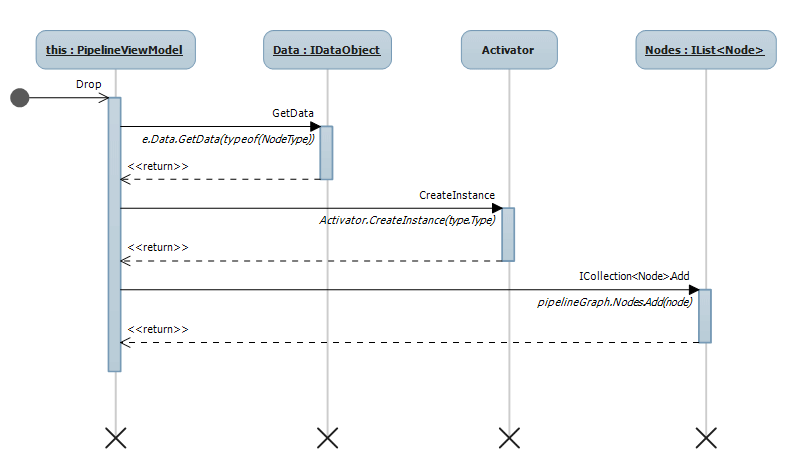
\includegraphics[height=0.7\textheight]{Diagrams/drop.png}
\end{center}
\end{figure}
\newpage

\begin{description}
	\item[Vorraussetzung] Das Programm ist gestartet.
	\item[äußerer Ablauf] Der Benutzer erzeugt einen beliebigen Knoten, indem er ihn per ``Drag-and-Drop'' aus einer am unteren Bildschirmrand angebrachten Leiste zieht.
	\item[innerer Ablauf] Durch das Platzieren des Knotens im Pipeline Graph wird ein Drop-Ereignis erzeugt. Dieses wird vom PipelineViewModel verarbeitet, indem zunächst die Art des platzierten Knotens erfasst und danach eine neue Instanz dieses Knotentyps erzeugt wird. Anschließend wird der neue Knoten zu der vom Pipeline Graph gehaltenen Liste der momentan vorhandenen Knoten hinzugefügt.
\end{description}
\newpage
\subsection{Hinzufügen eines Ausgabefensters}
\begin{figure}[h!]
\begin{center}
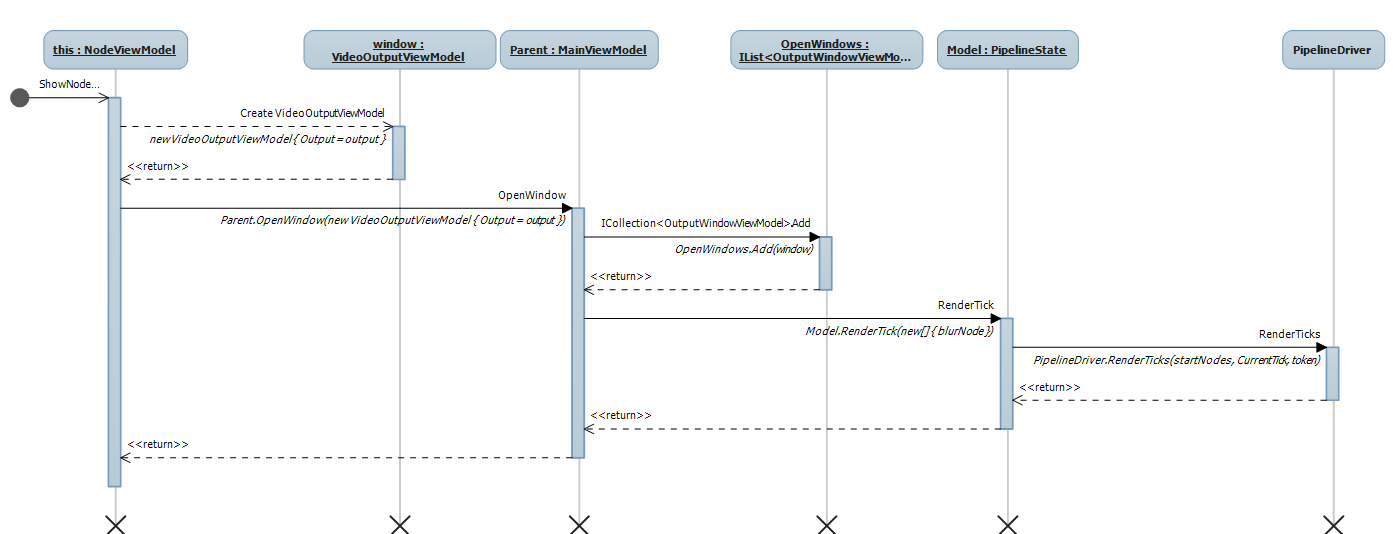
\includegraphics[height=0.9\textheight]{Diagrams/shownodeoutput.png}
\end{center}
\end{figure}
\newpage

\begin{figure}[h!]
\begin{center}
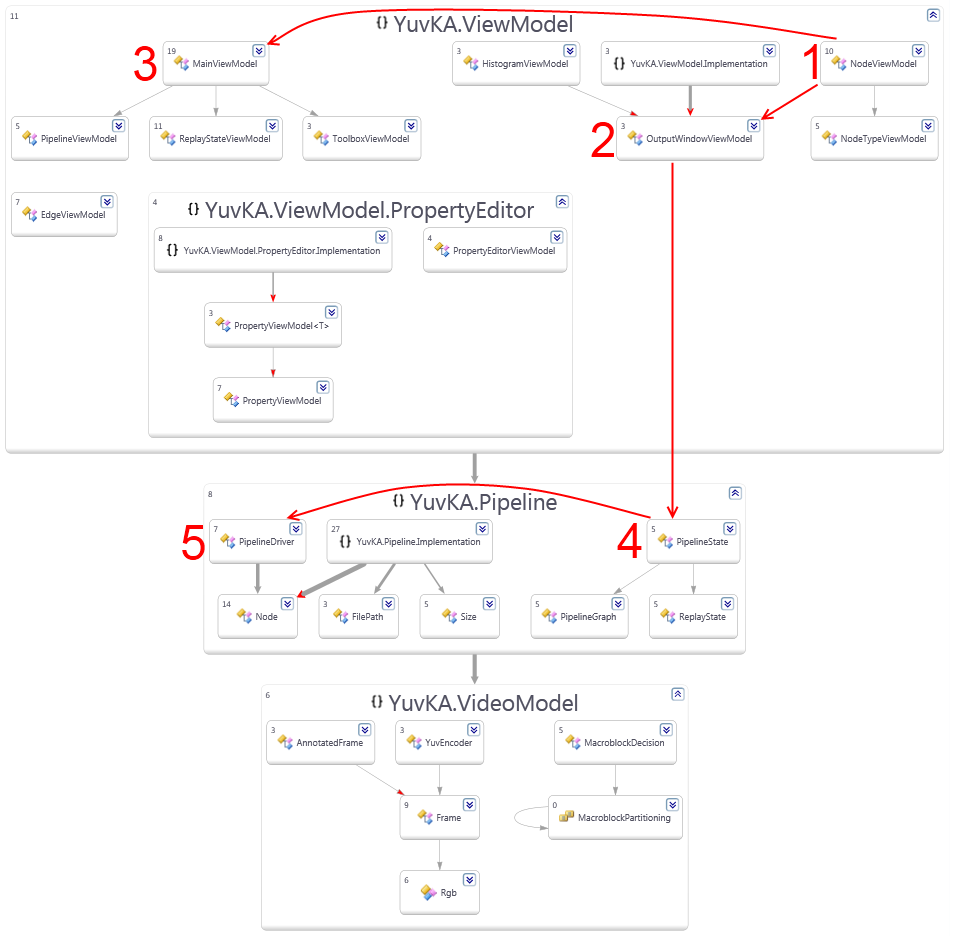
\includegraphics[width=0.9\textwidth]{Diagrams/visualization_TC2.png}
\end{center}
\caption{Veranschaulichung des Ablaufs anhand des Klassendiagramms}
\end{figure}
\begin{description}
	\item[Vorraussetzung] Der Benutzer hat eine Pipeline gebaut, die einen Weichzeichnungsknoten enthält.
	\item[äußerer Ablauf] Der Benutzer ruft das Kontextmenü des Weichzeichnungsknoten auf und wählt die Option ``Video anzeigen".
	\item[innerer Ablauf] Der Aufruf der Option wird vom NodeViewModel (1) verarbeitet. Dieses erstellt ein neues VideoOutput Fenster, verwaltet vom VideoOutputViewModel (2). Dieses Fenster wird vom MainViewModel (3) in dessen Liste aller geöffneten Fenster aufgenommen. Zum Abspielen ruft das MainViewModel die Klasse ReplayState (4) auf. Diese wiederum benutzt den PipelineDriver (5, siehe auch nächstes Diagramm) zum Verarbeiten des Videos.
\end{description}
\newpage
\subsection{Abspielen der Pipeline}
\begin{figure}[h!]
\begin{center}
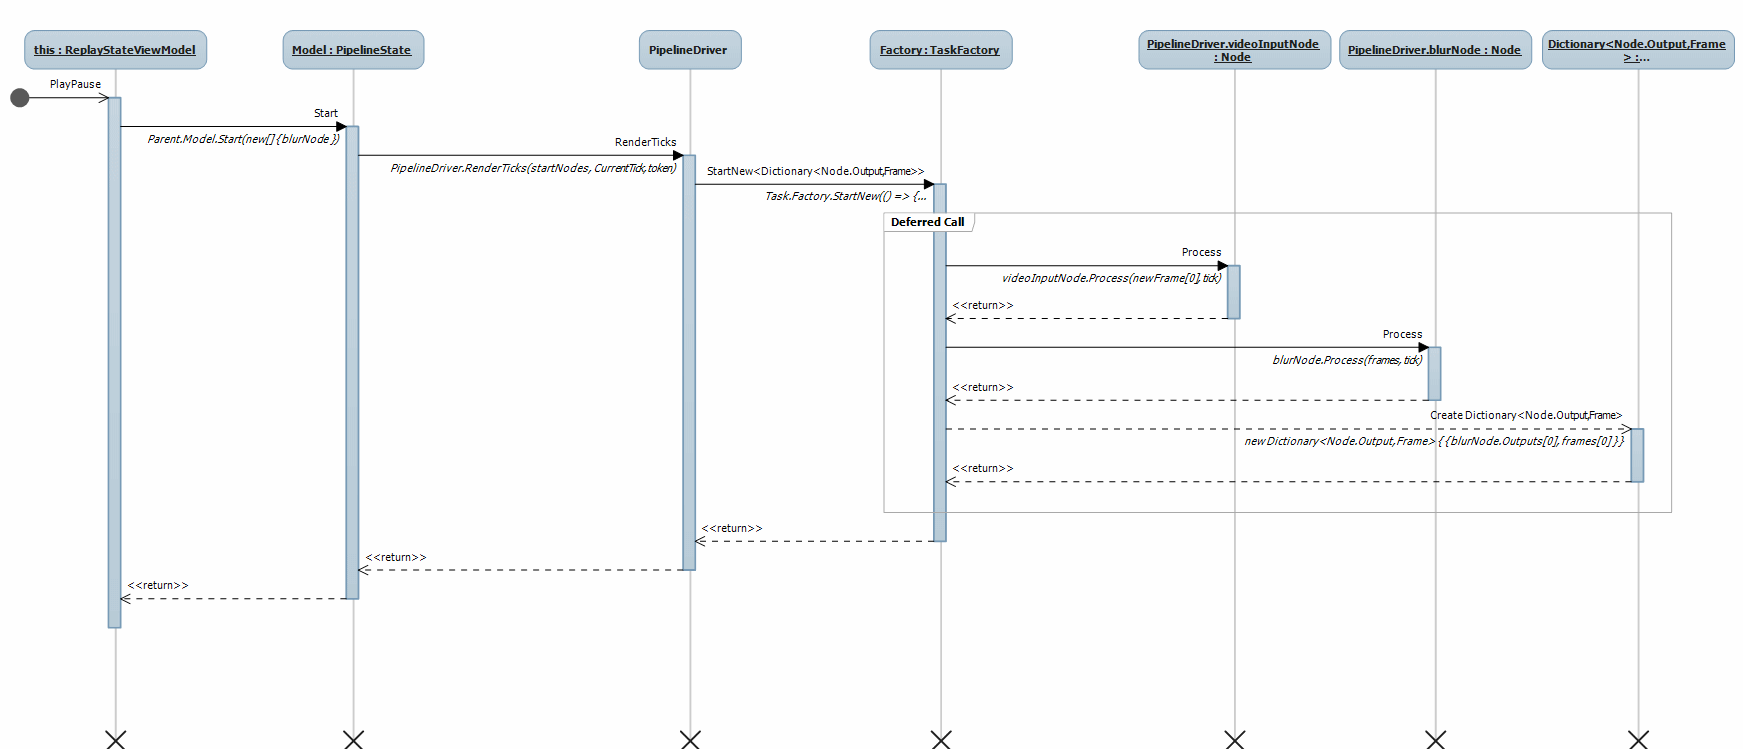
\includegraphics[height=0.9\textheight]{Diagrams/play.png}
\end{center}
\end{figure}
\newpage

\begin{figure}[h!]
\begin{center}
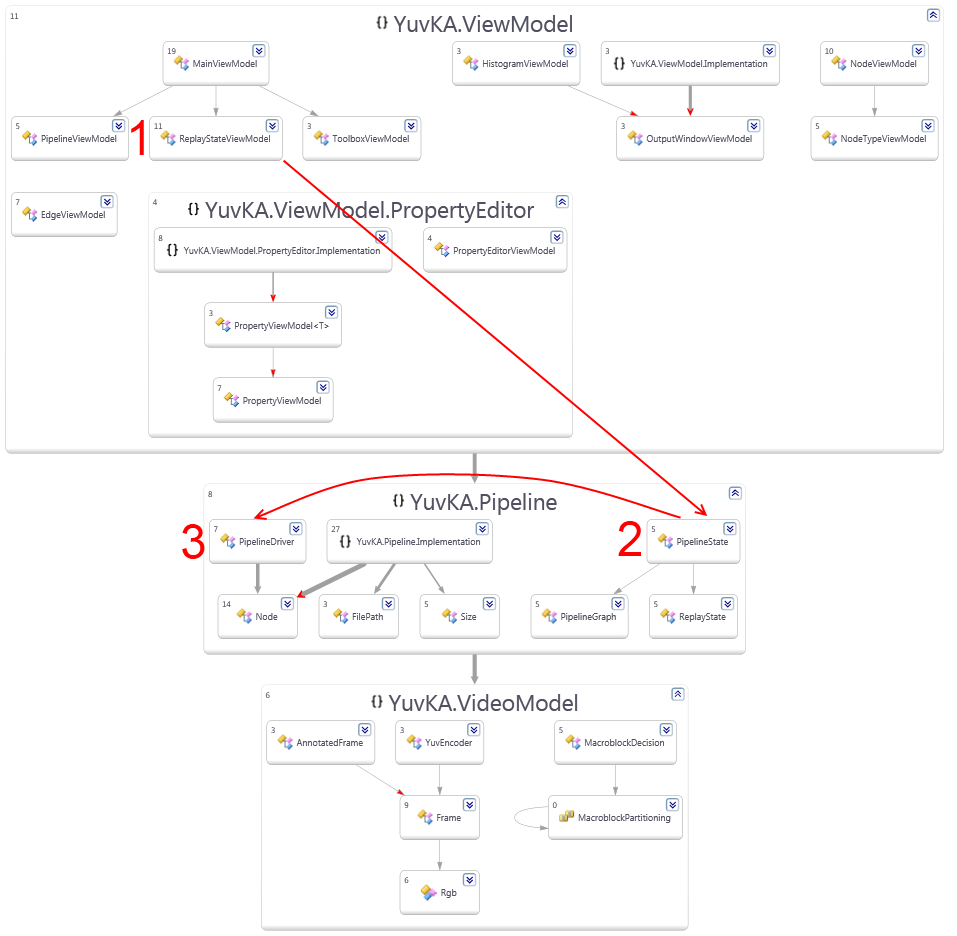
\includegraphics[width=0.9\textwidth]{Diagrams/visualization_TC3.png}
\end{center}
\caption{Veranschaulichung des Ablaufs anhand des Klassendiagramms}
\end{figure}
\begin{description}
	\item[Vorraussetzung] Der Benutzer hat eine Pipeline gebaut, die einen Weichzeichnungsknoten enthält und dessen Ausgabefenster geöffnet.
	\item[äußerer Ablauf] Der Benutzer drückt auf den Play-Knopf, um die Pipeline abzuspielen.
	\item[innerer Ablauf] Der Aufruf der Option wird vom ReplayStateViewModel (1) verarbeitet. Zum Abspielen ruft es  über das MainViewModel die Klasse ReplayState (2) auf. Diese wiederum benutzt den PipelineDriver (3) zum Verarbeiten des Videos. Der PipelineDriver verarbeitet die Frames, indem er für jeden Knoten einen Thread erstellt und diese nacheinander das Video abarbeiten lässt.
\end{description}


\section{Gantt-Diagramm}

\begin{figure}[h!]
\begin{center}
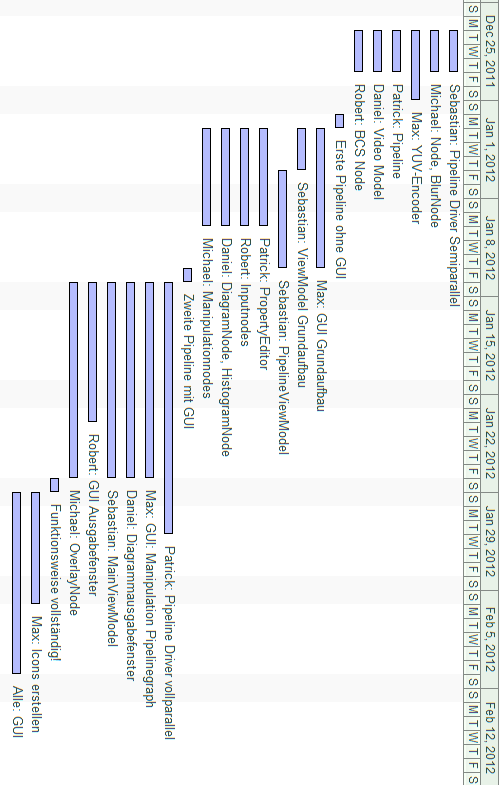
\includegraphics[height=0.7\textheight]{Diagrams/ganttchart.png}
\end{center}
\caption{Zeitplanung der Implementationsphase des Projektes als Gantt-Diagramm.}
\end{figure}

\section{Glossar}

\begin{description}
    \item[(Video-)Artefakte] Darstellungsfehler, welche sich dadurch zeigen, dass das enkodierte Video sichtlich stark von dem Referenzvideo abweicht
    \item[Asynchrone UI] Nichtblockend gestaltete Oberfläche, die bei Ladeoperationen weiterhin auf Interaktion reagiert
    \item[Differenzvideo] Videostream, welcher aus den Daten besteht, die bei der pixelweisen Subtraktion der Farbwerte zweier Videos entstehen
    \item[Drag-and-Drop] Bedienungsmuster, bei dem virtuelle Objekte mit der linken Maustaste ``gegriffen'' und ``gezogen'' werden
    \item[Farbkanal] Ein Farbbild besteht in der Regel aus 3 Farbkanälen, beispielsweise RGB (rot, grün, blau) oder \emph{YUV}.
    \item[Frame] Einzelbild eines Videos, bei \emph{H.264} unterteilt in \emph{Macroblöcke}
    \item[H.264] Weit verbreiteter \emph{Video-Codec} und Ziel-Codec der zu testenden Encoder
    \item[Histogramm] Diagrammart ähnlich einem Balkendiagramm, welche aber auch den Flächeninhalt eines Balken korrekt skaliert darstellt
    \item[Interface, UI] Benutzeroberfläche. Man unterscheidet zwischen Konsolenoberfläche und graphischer Oberfläche.
    \item[Inter-Frame] Videoframe, dessen Daten aus einem oder mehreren benachbarten Frames berechnet werden
    \item[Intra-Frame] Videoframe, dessen Daten unabhängig von denen anderer Frames gespeichert sind. Vergleiche \emph{Inter-Frame}.
    \item[Macroblock] Bei \emph{H.264} 16x16 Pixel große Blöcke, in die jeder \emph{Frame} aufgeteilt wird. Im Gegensatz zu älteren Codecs kann bei H.264 für jeden Macroblock eine unterschiedliche \emph{Inter/Intra-Frame}-Entscheidung getroffen werden. 
    \item[Move Vector] Vektor, um den jeder Referenzframe eines \emph{Inter-Frames} zusätzlich verschoben werden kann. Ermöglicht eine effiziente Kodierung von verschiebenden Bewegungen.
    \item[Multithreading] Programmiertechnik, in der die zu verrichtende Arbeit auf mehrere Prozessfäden verteilt wird. Dies ermöglicht Parallelismus und die optimale Auslastung von Multikern-Systemen
    \item[Noise] Ein randomisiertes Signal. Allgemein als ``Bildrauschen'' zu verstehen.
    \item[Overlay] Ein transparent über ein anderes Objekt gezeichnetes Objekt
    \item[Peak signal-to-noise ratio] Maß für den wahrgenommenen Qualitätsverlust eines komprimierten Videoframes
    \item[Pipeline] Hintereinanderschaltung von verschiedenen Knotentypen zum Einlesen, Modifizieren und Analysieren von Videos, in der UI dargestellt als Graph mit über \emph{Drag-and-Drop} erstellbaren Kanten
    \item[Resolution] Bildauflösung
    \item[Undo/Redo] ``Aktion zurücknehmen/wiederholen''
    \item[Video-Codec] Spezifikation eines Verfahrens, um Videodaten (meist verlustbehaftet) zu komprimieren
    \item[Videoencoder] Programm, welches rohe Videodaten als Eingabe annimmt und in einem bestimmten \emph{Video-Codec} entsprechendes Format bringt
    \item[YUV] Eine Familie von Farbpaletten, welche die Sehart des menschlichen Auges in Betracht nehmen
\end{description}


\end{document}
